\documentclass[%
11pt,%
%oneside,%
twoside,%
%twocolumn,%
titlepage,%
%fleqn,%
a4page,%
%ngerman,%
headsepline%
]{scrartcl}

%\usepackage{fancyhdr}
%\usepackage{scrpage2}
\usepackage{lastpage}
\usepackage{geometry}
\usepackage{graphicx}
\usepackage[utf8]{inputenc}
\usepackage[ngerman]{babel}
\usepackage{lscape}
\usepackage{mymath}
\usepackage{units}
\usepackage{nicefrac}
\usepackage{pgf,tikz}
%\usetikzlibrary{arrows}
\usepackage{colortbl}
\usepackage{hhline}
\usepackage{multirow}
\usepackage[extendedchars]{grffile}
\usepackage{caption}
\usepackage{multicol,calc}
\usepackage{blindtext}
\usepackage{pdfpages}
\usepackage{hyperref}
%\usepackage{tikz-er2}
\usepackage{framed}
\usetikzlibrary{arrows}
\usetikzlibrary{positioning}
\usetikzlibrary{shadows}

%\usepackage{romannum}
\usepackage{longtable}
\usepackage{listings}
\usepackage{wrapfig}


% Command, um Tabellen-Spalten anzupassen
\newcommand{\spaltenheight}{\rule{0mm}{3ex}}
\newcommand{\spaltenwidth}{\rule{3cm}{0mm}}
\newcommand{\spaltensep}{\\[1ex]}
%\arrayrulecolor{darkgreen}
\doublerulesepcolor{white}
\definecolor{lightyellow}{rgb}{1,1,0.8}
\definecolor{Gray}{gray}{0.9}


% Pagestyle/Layout
%\geometry{a4paper , tmargin =2.5cm,	bmargin=3cm, lmargin =2.5cm,	rmargin =2.5cm,	headheight=3em, headsep=1em, footskip=1cm}
\setlength{\parindent}{0pt} \setlength{\parskip}{1em}
%für TwoSide
%\lehead{\headmark\pagemark}
%\cehead{}
%\rehead{}
%\lohead{}
%\cohead{}
%\rohead{\headmark}
%für OneSide
%\ihead{}
%\chead{}
%\ohead{}
%\setheadsepline{0.5pt} % Linie zur Begrenzung
%\setfootsepline{0.5pt} % Linie zur Begrenzung
\pagestyle{headings} % gemachte Einstellungen anwenden


\subject{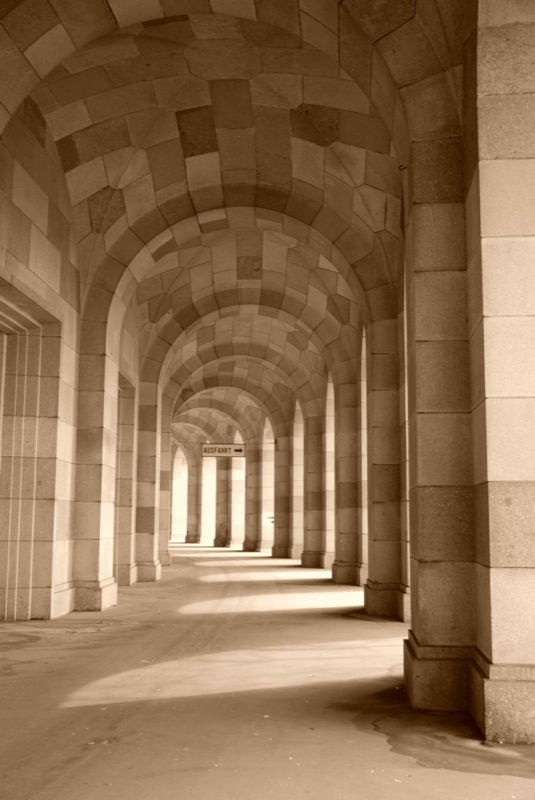
\includegraphics[width=0.618\textwidth]{pictures/torbogen.jpg}}
\title{Ähnlichkeit}
\subtitle{$k$, $k^2$ und $k^3$}
\author{}
\date{}
\lowertitleback{

\includegraphics[height=4ex]{pictures/gymfmslerbermattlogo.eps}\hfill
\includegraphics[height=4ex]{pictures/banner soft.png}}%
%\copyright Jorma Wassmer
%1. Auflage, Februar 2011
%}


\begin{document}
\maketitle

\cleardoublepage

\tableofcontents
%\thispagestyle{empty}
\cleardoublepage
%\setcounter{page}{1}

\section{Kongruenzabbildungen}
\begin{wrapfigure}{r}{0.382\textwidth}
  \begin{center}
    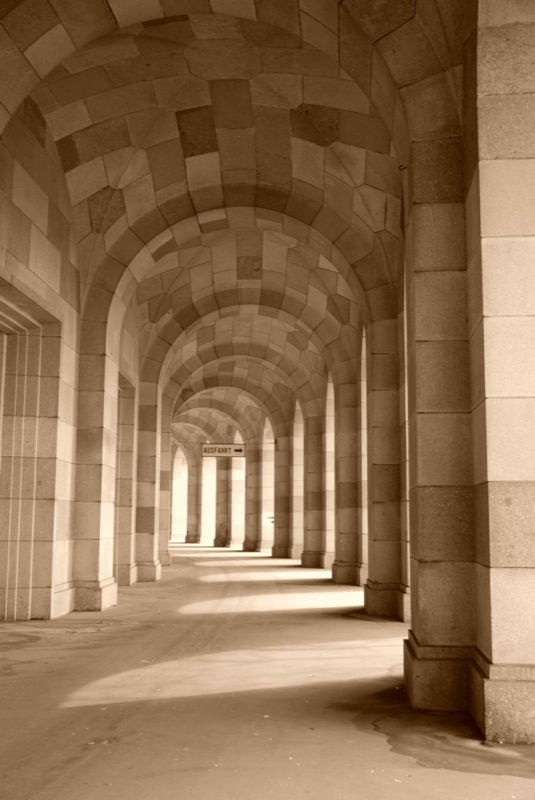
\includegraphics[width=0.382\textwidth]{pictures/torbogen}
  \end{center}
%\caption{A gull}
\end{wrapfigure}
Eine Abbildung ist eine eindeutige Zuordnung, bei der jedem Punkt einer ersten Punktmenge genau ein Punkt einer zweiten Punktmenge zugeordnet wird. Bei den Punktmengen handelt es sich um Geraden, Strecken, Winkel, Figuren (z.B. Dreiecke, Kreise), usw.

Wir nennen die erste Punktmenge die Originalmenge und die zweite Punktmenge die Bildmenge. In der Regel bezeichnen wir die Bildpunkte zu den Originalpunkten $A$, $B$, $P$, \dots\ mit $A'$, $B'$, $P'$, \dots.\\

Abbildungen, bei denen die Bildmenge deckungsgleich (kongruent) zur Originalmenge ist, heissen Kongruenzabbildungen. Kongruente Figuren haben also dieselbe Form und dieselbe Gr\"osse. Zu den Kongruenzabbildungen geh\"oren
\begin{itemize}
\item Achsenspiegelungen
\item Rotationen
\item Punktspiegelungen
\item Translationen
\item Verkettungen oben genannter Abbildungen
\end{itemize}

\begin{bsps}
\ \\[-2ex]
\begin{enumeratea}
\item Achsenspiegelung der Figur $F$ an der Geraden $g$%\\[4cm]
\item Drehung der Figur $F$ um den Drehpunkt $Z$ um den Winkel $\ga$%\\[5.5cm]
\item Punktspiegelung der Figur $F$ am Punkt $Z$%\\[6cm]
\item Verschiebung der Figur $F$ um einen vorgegebenen Verschiebungspfeil%\\[6cm]
\item Verkettung einer Achsenspiegelung mit einer Drehung
\end{enumeratea}
\end{bsps}

\section{Zentrische Streckung}
Wir w\"ahlen einen Punkt $Z$ der Ebene und eine positive Zahl $k$. Ordnen wir nun jedem Punkt $P$ einen Bildpunkt $P'$ zu gem\"ass der Vorschrift
\begin{itemize}
\item $P'$ liegt auf dem Strahl $ZP$
\item Die Strecke $ZP'$ ist $k$-mal so lang wie die Strecke $ZP$
\end{itemize}
so heisst diese Abbildung eine zentrische Streckung mit dem Streckungszentrum $Z$ und dem Streckungfaktor $k$.%\\[7cm]

F\"ur $k>1$ ist das Bild gr\"osser als das Original, f\"ur $k=1$ sind Bild und Original identisch und f\"ur $0<k<1$ ist das Bild kleiner als das Original.

\begin{bsp} Gegeben sind ein Punkt $Z$ und ein Dreieck $ABC$. Das Dreieck ist von $Z$ aus mit dem Streckungsfaktor $2$ zentrisch zu strecken.%\\[6cm]
\end{bsp}
Eine zentrische Streckung hat folgende Eigenschaften
\begin{itemize}
\item Originalwinkel und Bildwinkel sind gleich gross.
\item Originalgerade und Bildgerade sind parallel.
\item Die Bildstrecke ist $k$-mal so lang wie die Originalstrecke.
\item Der Fl\"acheninhalt der Bildfigur ist $k^2$-mal so gross wie der Fl\"acheninhalt der Originalfigur.
\end{itemize}

\begin{ueb}
Strecken Sie ein Quadrat $Q$ von einem Punkt $Z$ aus mit dem Streckungsfaktor $3$ zentrisch und \"uberpr\"ufe anschliessend obige Eigenschaften.%\\[8cm]
\end{ueb}

\begin{ueb}
Eine Streckung mit einem negativen Streckungsfaktor bedeutet eine Streckung mit dem entgegengesetzten positiven Streckungsfaktor und eine zus\"atzliche Punktspiegelung am Streckungszentrum.

\noindent Strecke ein Dreieck von $Z$ aus mit dem Streckungsfaktor $-\frac{1}{2}$.
\end{ueb}

\section{\"Ahnlichkeitsabbildungen}
Kongruenzabbildungen, zentrische Streckungen und ihre Verkettungen heissen \"Ahnlichkeitsabbildungen. Figuren, welche durch \"Ahnlichkeitsabbildungen auseinander hervorgehen, heissen zueinander \"ahnlich. \"Ahnliche Figuren haben dieselbe Form.

\begin{bsp}
Verkettung einer Drehung mit einer zentrischen Streckung.%\\[7cm]
\end{bsp}

Eine \"Ahnlichkeitsabbildung hat folgende Eigenschaften
\begin{itemize}
\item Originalwinkel und Bildwinkel sind gleich gross.
\item Alle Bildstrecken sind $k$-mal so lang wie die entsprechenden Originalstrecken.
\item Der Fl\"acheninhalt der Bildfigur ist $k^2$-mal so gross wie der Fl\"acheninhalt der Originalfigur
\end{itemize}
Daraus folgt insbesondere f\"ur \"ahnliche Dreiecke, dass sie gleiche Winkel haben und im Verh\"altnis von zwei einander entsprechenden Seiten \"ubereinstimmen.

\begin{ueb}
Alle Kreise sind zueinander \"ahnlich. Wie verhalten sich die Fl\"achen zweier Kreise, wenn sich ihre Radien wie $2\div3$ verhalten? Gib ein konkretes Beispiel zweier solcher Kreise.
\end{ueb}

\section{Strahlens\"atze}
\begin{satz}[1. Strahlensatz]
Werden zwei Strahlen mit gemeinsamem Anfangspunkt von zwei Parallelen geschnitten, so verhalten sich die Abschnitte auf dem einen Strahl wie die entsprechenden Abschnitte auf dem andern Strahl.%\\[6cm]
\end{satz}

\begin{bsp}
Standardbeispiel mit $a=25$, b=$10$ und $c=32$. Bestimme den fehlenden Abschnitt $d$.%\\[6cm]
\end{bsp}

\begin{ueb}
Teile eine Strecke im Verh\"altnis $2\div3$.
\end{ueb}

\begin{satz}[2. Strahlensatz]
Werden zwei Strahlen mit gemeinsamem Anfangspunkt von zwei Parallelen geschnitten, so verhalten sich die Parallelenabschnitte wie die vom Anfangspunkt aus gemessenen Abschnitte auf einem der Strahlen.%\\[6cm]
\end{satz}

\begin{bsp}
Standardbeispiel mit $a=8$, $b=3$ und $p=10$. Bestimme $q$.%\\[6cm]
\end{bsp}

\begin{ueb}
Eine freistehende Telefonstange im ebenen Gel\"ande wirft bei einem bestimmten Sonnenstand einen Schatten von $\unit[5.6]{m}$ L\"ange. Um die Stangenh\"ohe $h$ zu bestimmen, wird ein Meterstab parallel zur Stange aufgestellt, so dass beide Schattengrenzen zusammenfallen. Der Abstand des Meterstabes von der Stange misst $\unit[2.9]{m}$.
\end{ueb}

Beide Strahlens\"atze gelten sinngem\"ass auch dann, wenn \dots
\begin{itemize}
\item \dots\ mehr als zwei Strahlen von zwei Parallelen geschnitten werden.
\item \dots\ zwei Strahlen von mehr als zwei Parallelen geschnitten werden.
\item \dots\ anstatt Strahlen zwei sich schneidende Geraden von zwei Parallelen geschnitten werden.
\end{itemize}

\begin{bsp}
Ein Fotograf steht in der Entfernung $e=\unit[60]{m}$ von einem Baum. Die Brennweite $f$ des Kamera-Objektivs betr\"agt $\unit[45]{mm}$, die Gr\"osse $a$ des Baum-Bildes auf dem Negativ misst $\unit[24]{mm}$. Berechne die Baumh\"ohe $h$.%\\[7cm]
\end{bsp}
Alle Strahlens\"atze lassen sich z.B. mit Hilfe von \"ahnlichen Dreiecken beweisen.

\section{\"Ahnliche K\"orper}
K\"orper, welche durch \"Ahnlichkeitsabbildungen auseinander hervorgehen, heissen zueinander \"ahnlich. \"Ahnliche K\"orper haben dieselbe Form.

Neben den bereits bekannten Eigenschaften von \"Ahnlichkeitsabbildungen
\begin{itemize}
\item Eine Bildstrecke ist $k$-mal so lang wie die entsprechende Originalstrecke.
\item Der Fl\"acheninhalt einer Bildfigur ist $k^2$-mal so lang wie der Fl\"acheninhalt der entsprechenden Originalfigur.
\end{itemize}
gilt zus\"atzlich
\begin{itemize}
\item Das Volumen de Bildk\"orpers ist $k^3$-mal so gross wie das Volumen des Originalk\"orpers%\\[6cm]
\end{itemize}

\pagebreak

\begin{bsp}
Alle W\"urfel sind zueinander \"ahnlich.\\

\definecolor{wwwwww}{rgb}{0.4,0.4,0.4}
\begin{center}
\scalebox{1}{
\begin{tikzpicture}[line cap=round,line join=round,>=triangle 45,x=0.8259911894273128cm,y=0.6036217303822938cm]
\draw [color=wwwwww,dash pattern=on 2pt off 2pt, xstep=0.5cm,ystep=0.5cm] (-4.3,-3.8) grid (13.3,6.3);
\clip(-4.3,-3.64) rectangle (13.86,6.3);
\end{tikzpicture}
}
\end{center}
\end{bsp}

\begin{bsps}
\ \\[-2ex]
\begin{enumeratea}
\item Zwei W\"urfel aus gleichem Material wiegen $\unit[1]{g}$ und $\unit[1]{kg}$. Der leichtere W\"urfel hat eine Kantenl\"ange von $\unit[5]{cm}$. Wie lang ist eine Kante des schwereren W\"urfels?

Weil die beiden W\"urfel aus gleichem Material sind verhalten sich wegen
$$\frac{m_1}{m_2}=\frac{V_1\cdot\rho}{V_2\cdot\rho}=\frac{V_1}{V_2}$$
ihre Volumina wie $1\div1000$, also wegen $10^3=1000$ ihre Kantenl\"angen wie $1\div10$. Die Kantenl\"ange des schwereren W\"urfels betr\"agt deshalb $\unit[50]{cm}$.
\item Ein gerader Kreiskegel wird durch einen Schnitt parallel zur Grundfl\"ache in halber H\"ohe geteilt. Er zerf\"allt dabei in einen kleineren Kegel und einen Kegelstumpf. Wie verhalten sich die Volumina der beiden Teile?

Der kleine Kegel ist zum urspr\"unglichen \"ahnlich (zentrische Streckung mit Kegelspitze als Streckungszentrum). Ihre H\"ohne verhalten sich wie $1\div2$, ihre Grundfl\"achen wie $1\div4$ und ihre Volumina wie $1\div8$. Das Volumen des Kegelstumpfs ist Volumen des urspr\"unglichen Kegels minus Volumen des kleinen Kegels. Also verh\"alt sich das Volumen des kleinen Kegels zu dem des Kegelstumpfs wie $1\div7$.
\end{enumeratea}
\end{bsps}

\pagebreak

\vspace*{-2ex}

\section{\"Ubungen}
\begin{enumerate}
\item Spiegle das Dreieck und den Kreis an der Geraden $g$.\\
\begin{center}
\scalebox{1.3}{
\begin{tikzpicture}[line cap=round,line join=round,>=triangle 45,x=0.7cm,y=0.7cm]
\clip(-4.22,-3.2) rectangle (6.84,5.64);
\draw [line width=1.6pt,domain=-4.22:6.84] plot(\x,{(--18.3-3.62*\x)/10.7});
\draw [line width=2pt] (0.96,1.39)-- (-0.58,5.4);
\draw [line width=2pt] (-0.58,5.4)-- (-0.72,1.1);
\draw [line width=2pt] (-0.72,1.1)-- (0.96,1.39);
\draw [line width=1.6pt] (3.6,-1.7) circle (0.8cm);
\draw[color=black] (-3.24,2.36) node {$g$};
\fill [color=black] (3.6,-1.7) circle (1.5pt);
\end{tikzpicture}
}
\end{center}
\item Die Figur $F$ kann durch eine Achsenspiegelung in die Figur $F'$ \"uberf\"uhrt werden. Konstruiere die Spiegelachse.\\
\begin{center}
\scalebox{1.2}{
\begin{tikzpicture}[line cap=round,line join=round,>=triangle 45,x=1cm,y=1cm]
\clip(-3.17,-2.47) rectangle (4.08,2.91);
\draw [line width=1.6pt] (-1.98,-1.86)-- (-2.22,-0.14);
\draw [line width=1.6pt] (-2.22,-0.14)-- (0.64,-2.18);
\draw [line width=1.6pt] (3.33,1.56)-- (1.86,2.49);
\draw [line width=1.6pt] (1.86,2.49)-- (2.54,-0.96);
\draw (-2.79,-0.69) node[anchor=north west] {$F'$};
\draw (3.1,2.3) node[anchor=north west] {$F$};
\end{tikzpicture}
}
\end{center}



\item Spiegle das Rechteck $ABCD$ an der Rechteckdiagonalen durch $A$ und $C$.\\
\begin{center}
\scalebox{1.2}{
\begin{tikzpicture}[line cap=round,line join=round,>=triangle 45,x=0.9cm,y=0.9cm]
\clip(-2.66,-2.21) rectangle (3.98,1.08);
\draw [line width=2pt] (-1.87,-1.32)-- (2.91,-1.32);
\draw [line width=2pt] (2.91,-1.32)-- (2.86,0.52);
\draw [line width=2pt] (2.86,0.52)-- (-1.87,0.48);
\draw [line width=2pt] (-1.87,0.48)-- (-1.87,-1.32);
\draw (-2.1,-1.4) node[anchor=north west] {$A$};
\draw (2.6,-1.4) node[anchor=north west] {$B$};
\draw (2.6,1) node[anchor=north west] {$C$};
\draw (-2.1,1) node[anchor=north west] {$D$};
\end{tikzpicture}
}
\end{center}

\item Geht eine Figur durch eine Achsenspiegelung in sich selbst \"uber, so heisst die Figur achsensymmetrisch. Bei Achsensymmetrie heisst die Spiegelachse auch Symmetrieachse der Figur.

Zeichne bei den Figuren alle m\"oglichen Symmetrieachsen und Symmetriepunkte ein.\\
\begin{center}
\scalebox{1.1}{
\begin{tikzpicture}[line cap=round,line join=round,>=triangle 45,x=0.9cm,y=0.75cm]
\clip(-4.7,-0.9) rectangle (8,2.84);
\draw [line width=2pt] (-4,2)-- (-1,2);
\draw [line width=2pt] (-1,2)-- (-1,0);
\draw [line width=2pt] (-1,0)-- (-4,0);
\draw [line width=2pt] (-4,0)-- (-4,2);
\draw [line width=2pt] (1,-0.5)-- (1,1.5);
\draw [line width=2pt] (1,1.5)-- (4,2.5);
\draw [line width=2pt] (4,2.5)-- (4,0.5);
\draw [line width=2pt] (4,0.5)-- (1,-0.5);
\draw [line width=2pt] (5,2)-- (7,2);
\draw [line width=2pt] (7,2)-- (7,0);
\draw [line width=2pt] (7,0)-- (5,0);
\draw [line width=2pt] (5,0)-- (5,2);
\end{tikzpicture}
}
\end{center}
\item Drehe den Punkt $P$ um $Z$ um den Winkel $120^\circ$ im Uhrzeigersinn.\\[4cm]
\begin{center}
\scalebox{1.1}{
\begin{tikzpicture}[line cap=round,line join=round,>=triangle 45,x=1.368cm,y=1.368cm]
\clip(-2.66,-0.56) rectangle (3.92,1.08);
\fill [color=black] (-1.39,0.3) circle (1.5pt);
\draw[color=black] (-1.27,0.52) node {$P$};
\fill [color=black] (1.67,0.25) circle (1.5pt);
\draw[color=black] (1.78,0.47) node {$Z$};
\end{tikzpicture}
}
\end{center}
\item Drehe die Figur im Gegenuhrzeigersinn um $Z$ um den Winkel $\ga$.\\
\begin{center}
\definecolor{qqwuqq}{rgb}{0,0.39,0}
\scalebox{0.95}{
\begin{tikzpicture}[line cap=round,line join=round,>=triangle 45,x=1.0817369093231162cm,y=1.0783987915407858cm]
\clip(-2.66,-4.39) rectangle (10.28,1.08);
\draw [shift={(9.42,-2.04)},line width=1pt,color=qqwuqq] (0,0) -- (130.66:0.83) arc (130.66:226.37:0.83) -- cycle;
\draw [line width=2pt] (0.94,-0.62)-- (-1.04,-2.21);
\draw [line width=2pt] (-1.04,-2.21)-- (0.48,-3.25);
\draw [line width=2pt] (0.48,-3.25)-- (0.94,-0.62);
\draw (8.31,-0.76)-- (9.42,-2.04);
\draw (8.41,-3.1)-- (9.42,-2.04);
\fill [color=black] (3.01,-1.32) circle (1.5pt);
\draw[color=black] (3.12,-1.1) node {$Z$};
\draw[color=qqwuqq] (8.9,-2) node {$\alpha$};
\end{tikzpicture}
}
\end{center}

\item Die Aufnahme zeigt den n\"achtlichen Nordhimmel. Wegen der langen Belichtungszeit haben die Sterne kreisbogenf\"ormige Spuren hinterlassen, deren Mittelpunkt den Himmelspol kennzeichnet. Die dicke Spur unterhalb des Drehzentrums stammt vom Polarstern.

Wie lange wurde der Film belichtet?\\
\begin{center}
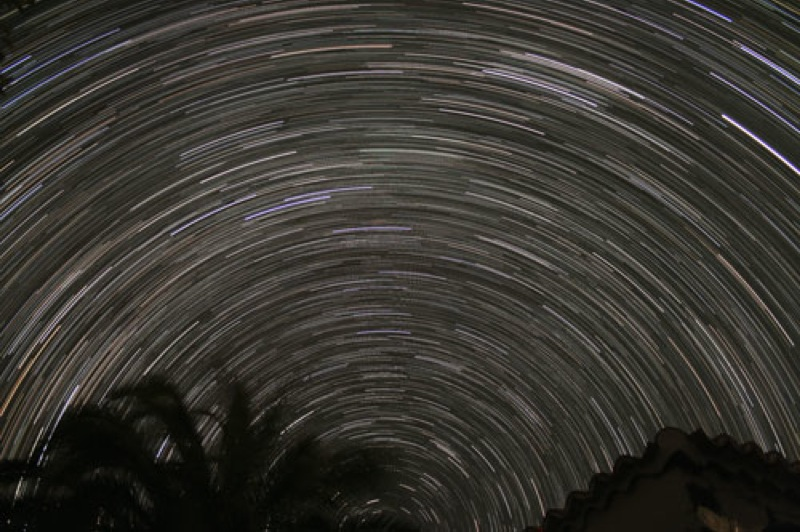
\includegraphics[width=0.92\textwidth]{pictures/ueb7}
\end{center}

\pagebreak

\item Der Punkt $A$ wurde um einen Drehpunkt nach $A'$ gedreht. Wo muss der Drehpunkt liegen?
\begin{center}
\scalebox{1}{
\begin{tikzpicture}[line cap=round,line join=round,>=triangle 45,x=0.7974481658692185cm,y=0.7943925233644861cm]
\clip(-4.3,2.02) rectangle (8.24,6.3);
\fill [color=black] (-2,3) circle (1.5pt);
\draw[color=black] (-1.84,3.4) node {$A$};
\fill [color=black] (4.56,3.84) circle (1.5pt);
\draw[color=black] (4.74,4.26) node {$A'$};
\end{tikzpicture}
}
\end{center}

\item Die Strecke $AB$ wurde um einen Drehpunkt nach $A'B'$ gedreht. Konstruiere den Drehpunkt.\\
\begin{center}
\scalebox{0.8}{
\begin{tikzpicture}[line cap=round,line join=round,>=triangle 45,x=0.75cm,y=0.75cm]
\clip(-4.3,-1.54) rectangle (7.86,6.3);
\draw [line width=2pt] (-2.16,0.22)-- (-0.42,3.98);
\draw [line width=2pt] (6.1,0.82)-- (3.58,4.1);
\draw (-2.8,0.8) node[anchor=north west] {$A$};
\draw (-0.9,4.68) node[anchor=north west] {$B$};
\draw (3.68,4.8) node[anchor=north west] {$A'$};
\draw (6.26,1.24) node[anchor=north west] {$B'$};
\end{tikzpicture}
}
\end{center}

\item Eine rechteckige Tischplatte soll auf ihrem Untergestell derart gelagert sein, dass sie die beiden gezeichneten Lagen einnehmen kann. An welcher Stelle muss der Tischler den Drehzapfen anbringen?\\
\begin{center}
\begin{tikzpicture}[line cap=round,line join=round,>=triangle 45,x=0.75cm,y=0.75cm]
\clip(-3.96,-0.84) rectangle (5.4,6.72);
\draw [line width=2pt] (-3,0)-- (3,0);
\draw [line width=2pt] (3,0)-- (3,2);
\draw [line width=2pt] (3,2)-- (-3,2);
\draw [line width=2pt] (-3,2)-- (-3,0);
\draw [line width=2pt,dash pattern=on 4pt off 4pt] (-1,6)-- (1,6);
\draw [line width=2pt,dash pattern=on 4pt off 4pt] (1,6)-- (1,0);
\draw [line width=2pt,dash pattern=on 4pt off 4pt] (1,0)-- (-1,0);
\draw [line width=2pt,dash pattern=on 4pt off 4pt] (-1,0)-- (-1,6);
\end{tikzpicture}
\end{center}

\pagebreak

\item Drehe die Figur um $Z$ um $180^\circ$.\\
\begin{center}
\begin{tikzpicture}[line cap=round,line join=round,>=triangle 45,x=0.8cm,y=0.8cm]
\clip(-3.76,-0.28) rectangle (4.86,5.12);
\draw [line width=2pt] (-2.22,4.54)-- (-3.42,0.46);
\draw [line width=2pt] (-3.42,0.46)-- (0.6,0.48);
\draw [line width=2pt] (0.6,0.48)-- (-0.1,3.58);
\draw [line width=2pt] (-0.1,3.58)-- (-2.22,4.54);
\fill [color=black] (4.14,1) circle (1.5pt);
\draw[color=black] (4.4,1.3) node {$Z$};
\end{tikzpicture}
\end{center}
\item Verschiebe das Dreieck um den vorgegebenen Verschiebungspfeil.\\[3ex]
\begin{center}
\scalebox{0.95}{
\begin{tikzpicture}[line cap=round,line join=round,>=triangle 45,x=0.79cm,y=0.79cm]
\clip(-3.76,-1.46) rectangle (8.92,5.12);
\draw [line width=2pt] (7.04,3.22)-- (7.68,-0.52);
\draw [line width=2pt] (7.68,-0.52)-- (5.5,-0.94);
\draw [line width=2pt] (5.5,-0.94)-- (7.04,3.22);
\draw [->] (7.04,3.22) -- (1.22,4.4);
\end{tikzpicture}
}
\end{center}

\item Das Viereck $V$ kann durch eine Verschiebung in $V'$ \"uberf\"uhrt werden. Zeichne einen zugeh\"origen Verschiebungspfeil.\\
\begin{center}
\scalebox{0.8}{
\begin{tikzpicture}[line cap=round,line join=round,>=triangle 45,x=1.0cm,y=1.0cm]
\clip(-2.6,-2.3) rectangle (7.28,3.58);
\draw [line width=2pt] (-1.38,1.02)-- (1.8,1.02);
\draw [line width=2pt] (1.8,1.02)-- (1.2,3.2);
\draw [line width=2pt] (1.2,3.2)-- (-0.72,2.7);
\draw [line width=2pt] (-0.72,2.7)-- (-1.38,1.02);
\draw [line width=1.6pt] (2.68,-1.24)-- (5.86,-1.24);
\draw [line width=1.6pt] (5.86,-1.24)-- (5.26,0.94);
\draw [line width=1.6pt] (5.26,0.94)-- (3.34,0.44);
\draw [line width=1.6pt] (3.34,0.44)-- (2.68,-1.24);
\draw (0.2,2.42) node[anchor=north west] {$V$};
\draw (4.28,0.1) node[anchor=north west] {$V'$};
\end{tikzpicture}
}
\end{center}

\pagebreak

\item Verschieben Sie das Dreieck zuerst um den ersten, dann um den zweiten angegebenen Verschiebungspfeil. Zeichnen Sie anschliessend einen Verschiebungspfeil, durch den das Originaldreieck direkt in die Endlage \"uberf\"uhrt wird.\\[-4ex]
\begin{center}

\begin{tikzpicture}[line cap=round,line join=round,>=triangle 45,x=0.94cm,y=0.94cm]
\clip(-4.3,0.12) rectangle (6.3,6.3);
\draw [line width=2pt] (-3.6,3.52)-- (-0.5,3.04);
\draw [line width=1.6pt] (-0.5,3.04)-- (-3.36,1.8);
\draw [line width=1.6pt] (-3.36,1.8)-- (-3.6,3.52);
\draw [->,line width=1pt] (-0.5,3.04) -- (4.8,3.82);
\draw [->,line width=1pt] (4.8,3.82) -- (5.16,2);
\end{tikzpicture}
\end{center}
\item Ein Sportflugzeug fliegt mit einer Geschwindigkeit von $\unitfrac[240]{km}{h}$ nach Norden. Von Westen weht ein Wind mit $\unitfrac[60]{km}{h}$. Bestimmen Sie an der Abbildung die Richtung und die tats\"achliche Geschwindigkeit des Flugzeugs gegen\"uber dem Erdboden.\\
\begin{center}
\scalebox{0.95}{
\begin{tikzpicture}[line cap=round,line join=round,>=triangle 45,x=1.04cm,y=1.04cm]
\clip(-1.12,-0.16) rectangle (1.76,4.3);
\draw [->,line width=1.6pt] (0,0) -- (1,0);
\draw [->,line width=1.6pt] (0,0) -- (0,4);
\draw (0.1,4) node[anchor=north west] {$\unitfrac[240]{km}{h}$};
\draw (0.4,0.7) node[anchor=north west] {$\unitfrac[60]{km}{h}$};
\end{tikzpicture}
}
\end{center}

\item Zwei Schlepper ziehen an einem Frachtschiff mit den Kr\"aften $F_1$ bzw.~$F_2$. Zeichne die resultierende Kraft, durch welche das Schiff bewegt wird.\\
\begin{center}
\definecolor{zzttqq}{rgb}{0.6,0.2,0}
\scalebox{0.7}{
\begin{tikzpicture}[line cap=round,line join=round,>=triangle 45,x=1.25cm,y=1.25cm]
\clip(-1.62,-1.18) rectangle (3.96,1.82);
\fill[color=zzttqq,fill=zzttqq,fill opacity=0.1] (-1.44,1.18) -- (-0.38,1.2) -- (-0.36,0.28) -- (-1.44,0.28) -- cycle;
\draw [->,line width=2pt] (0.88,0.78) -- (2.9,1.2);
\draw [->,line width=2pt] (0.88,0.78) -- (3.2,-0.48);
\draw (2.08,1.8) node[anchor=north west] {$F_1$};
\draw (2.3,-0.3) node[anchor=north west] {$F_2$};
\draw [shift={(-1.03,-2.21)},line width=2pt]  plot[domain=0.83:1.68,variable=\t]({1*3.95*cos(\t r)+0*3.95*sin(\t r)},{0*3.95*cos(\t r)+1*3.95*sin(\t r)});
\draw [shift={(-0.68,3)},line width=2pt]  plot[domain=4.46:5.5,variable=\t]({1*3.24*cos(\t r)+0*3.24*sin(\t r)},{0*3.24*cos(\t r)+1*3.24*sin(\t r)});
\draw [color=zzttqq] (-1.44,1.18)-- (-0.38,1.2);
\draw [color=zzttqq] (-0.38,1.2)-- (-0.36,0.28);
\draw [color=zzttqq] (-0.36,0.28)-- (-1.44,0.28);
\end{tikzpicture}
}
\end{center}

\pagebreak

\item Ein Schiff f\"ahrt bei einem Nordostwind von $\unitfrac[40]{km}{h}$ mit der Geschwindigkeit $\unitfrac[25]{km}{h}$ nach S\"uden. Von welcher Seite scheint f\"ur einen an Deck stehenden Passagier der Wind zu kommen und welche Geschwindigkeit scheint er zu haben? L\"ose die Aufgabe zeichnerisch.
\item Durch zentrische Streckung mit dem Streckungszentrum $Z$ ist aus dem Originaldreieck $ABC$ das Bilddreieck $A'B'C'$ entstanden.

Mit welchem Streckungsfaktor wurde es gestreckt? In welchem Verh\"altnis stehen entsprechende Seitenl\"angen zueinander? In welchem Verh\"altnis stehen die Fl\"acheninhalte zueinander?\\[-6ex]
\begin{center}
\definecolor{zzttqq}{rgb}{0.6,0.2,0}
\definecolor{wwttqq}{rgb}{0.4,0.2,0}
\definecolor{qqwwcc}{rgb}{0,0.4,0.8}
\definecolor{qqqqzz}{rgb}{0,0,0.6}
\begin{tikzpicture}[line cap=round,line join=round,>=triangle 45,x=0.865cm,y=0.865cm]
\clip(-1.62,-4.9) rectangle (9.94,1.82);
\fill[color=qqwwcc,fill=qqwwcc,fill opacity=0.1] (1.14,-1.62) -- (2.58,-1.92) -- (2.04,-2.58) -- cycle;
\fill[color=zzttqq,fill=zzttqq,fill opacity=0.1] (4.86,-0.66) -- (9.18,-1.56) -- (7.56,-3.54) -- cycle;
\draw [line width=2.4pt,color=qqwwcc] (1.14,-1.62)-- (2.58,-1.92);
\draw [line width=2.8pt,color=qqwwcc] (2.58,-1.92)-- (2.04,-2.58);
\draw [line width=2.4pt,color=qqwwcc] (2.04,-2.58)-- (1.14,-1.62);
\draw [domain=-0.72:9.94] plot(\x,{(-3.56--0.48*\x)/1.86});
\draw [domain=-0.72:9.94] plot(\x,{(-6.8--0.18*\x)/3.3});
\draw [domain=-0.72:9.94] plot(\x,{(-6.14-0.48*\x)/2.76});
\draw [line width=2.4pt,color=zzttqq] (4.86,-0.66)-- (9.18,-1.56);
\draw [line width=2.4pt,color=zzttqq] (9.18,-1.56)-- (7.56,-3.54);
\draw [line width=2.4pt,color=zzttqq] (7.56,-3.54)-- (4.86,-0.66);
\fill [color=black] (-0.72,-2.1) circle (1.5pt);
\draw[color=black] (-0.92,-1.7) node {$Z$};
\fill [color=qqqqzz] (1.14,-1.62) circle (1.5pt);
\draw[color=qqqqzz] (1.18,-1.26) node {$C$};
\fill [color=qqqqzz] (2.58,-1.92) circle (1.5pt);
\draw[color=qqqqzz] (2.72,-1.66) node {$B$};
\fill [color=qqqqzz] (2.04,-2.58) circle (1.5pt);
\draw[color=qqqqzz] (1.88,-2.86) node {$A$};
\fill [color=wwttqq] (4.86,-0.66) circle (1.5pt);
\draw[color=wwttqq] (5,-0.3) node {$C'$};
\fill [color=wwttqq] (9.18,-1.56) circle (1.5pt);
\draw[color=wwttqq] (9.36,-1.3) node {$B'$};
\fill [color=wwttqq] (7.56,-3.54) circle (1.5pt);
\draw[color=wwttqq] (7.44,-3.86) node {$A'$};
\end{tikzpicture}
\end{center}
\item Strecke die Figur von $Z$ aus mit dem Streckungsfaktor $\frac{1}{3}$.\\
\begin{center}
\definecolor{zzttqq}{rgb}{0.6,0.2,0}
\scalebox{1.1}{
\begin{tikzpicture}[line cap=round,line join=round,>=triangle 45,x=0.865cm,y=0.865cm]
\clip(-1.62,-4.9) rectangle (9.94,1.82);
\fill[color=zzttqq,fill=zzttqq,fill opacity=0.1] (-1.02,-2.56) -- (-0.98,-4.7) -- (5.1,-4.74) -- (5.1,-4.02) -- (-0.16,-4.02) -- (-0.2,-2.56) -- cycle;
\draw [color=zzttqq] (-1.02,-2.56)-- (-0.98,-4.7);
\draw [color=zzttqq] (-0.98,-4.7)-- (5.1,-4.74);
\draw [color=zzttqq] (5.1,-4.74)-- (5.1,-4.02);
\draw [color=zzttqq] (5.1,-4.02)-- (-0.16,-4.02);
\draw [color=zzttqq] (-0.16,-4.02)-- (-0.2,-2.56);
\draw [color=zzttqq] (-0.2,-2.56)-- (-1.02,-2.56);
\fill [color=black] (8.92,0.9) circle (1.5pt);
\draw[color=black] (8.7,1.26) node {$Z$};
\end{tikzpicture}
}
\end{center}

\pagebreak

\item Strecke das Rechteck von $Z$ aus mit dem Streckungsfaktor $-2$.\\
\begin{center}
\definecolor{zzttqq}{rgb}{0.6,0.2,0}
\definecolor{zzzzzz}{rgb}{0.6,0.6,0.6}
\scalebox{0.9}{
\begin{tikzpicture}[line cap=round,line join=round,>=triangle 45,x=0.93cm,y=0.93cm]
\draw [color=zzzzzz,dash pattern=on 2pt off 2pt, xstep=0.93cm,ystep=0.93cm] (0.56,-6.52) grid (15.62,1.4);
\clip(0.56,-6.52) rectangle (15.62,1.4);
\fill[color=zzttqq,fill=zzttqq,fill opacity=0.1] (3,0) -- (7,0) -- (7,-2) -- (3,-2) -- cycle;
\draw [color=zzttqq] (3,0)-- (7,0);
\draw [color=zzttqq] (7,0)-- (7,-2);
\draw [color=zzttqq] (7,-2)-- (3,-2);
\draw [color=zzttqq] (3,-2)-- (3,0);
\fill [color=black] (7,-2) circle (1.5pt);
\draw[color=black] (6.8,-2.32) node {$Z$};
\end{tikzpicture}
}
\end{center}
\item Das Dreieck $ABC$ kann durch eine zentrische Streckung in das Bilddreieck $A'B'C'$ \"uberf\"uhrt werden. Konstruiere das Streckungszentrum $Z$ und gib den Streckungsfaktor an.\\
\begin{center}
\definecolor{uququq}{rgb}{0.25,0.25,0.25}
\definecolor{zzttqq}{rgb}{0.6,0.2,0}
\definecolor{wwwwww}{rgb}{0.4,0.4,0.4}
\scalebox{0.9}{
\begin{tikzpicture}[line cap=round,line join=round,>=triangle 45,x=1.1cm,y=1.1cm]
\draw [color=wwwwww,dash pattern=on 3pt off 3pt, xstep=1.1cm,ystep=1.1cm] (0.56,-6.78) grid (14.28,1.4);
\clip(0.56,-6.78) rectangle (14.28,1.4);
\draw [line width=2pt,color=zzttqq] (3,-5)-- (10,-5);
\draw [line width=2pt,color=zzttqq] (10,-5)-- (5,-1);
\draw [line width=2pt,color=zzttqq] (5,-1)-- (3,-5);
\draw [line width=2pt] (2,-5.5)-- (12.5,-5.5);
\draw [line width=2pt] (12.5,-5.5)-- (5,0.5);
\draw [line width=2pt] (5,0.5)-- (2,-5.5);
\fill [color=zzttqq] (3,-5) circle (1.5pt);
\draw[color=zzttqq] (2.98,-5.26) node {$A$};
\fill [color=zzttqq] (10,-5) circle (1.5pt);
\draw[color=zzttqq] (9.98,-5.26) node {$B$};
\fill [color=zzttqq] (5,-1) circle (1.5pt);
\draw[color=zzttqq] (5.24,-0.82) node {$C$};
\fill [color=uququq] (2,-5.5) circle (1.5pt);
\draw[color=uququq] (2,-5.84) node {$A'$};
\fill [color=uququq] (12.5,-5.5) circle (1.5pt);
\draw[color=uququq] (12.52,-5.82) node {$B'$};
\fill [color=uququq] (5,0.5) circle (1.5pt);
\draw[color=uququq] (5.38,0.64) node {$C'$};
\end{tikzpicture}
}
\end{center}

\pagebreak

\item Verbindet man die Seitenmitten eines Dreiecks $ABC$, so entsteht ein weiteres Dreieck. Dieses k\"onnte aus dem Dreieck $ABC$ durch eine zentrische Streckung erhalten werden. Wo liegt das Streckungszentrum und wie gross ist der Streckungsfaktor?

\item Der Eckpunkt $B$ des Dreiecks $ABC$ wurde durch eine zentrische Streckung von $Z$ aus in $B'$ \"uberf\"uhrt. Konstruiere das Bilddreieck $A'B'C'$, und bestimme den Streckungsfaktor.\\
\begin{center}
\definecolor{uququq}{rgb}{0.25,0.25,0.25}
\definecolor{zzttqq}{rgb}{0.6,0.2,0}
\scalebox{0.95}{
\begin{tikzpicture}[line cap=round,line join=round,>=triangle 45,x=0.9336cm,y=0.9336cm]
\clip(0.56,-9.62) rectangle (10.2,1.4);
\draw [line width=2pt,color=zzttqq] (9,-3)-- (2,1);
\draw [line width=2pt,color=zzttqq] (2,1)-- (3,-3);
\draw [line width=2pt,color=zzttqq] (3,-3)-- (9,-3);
\draw (2,1)-- (2,-9);
\fill [color=black] (9,-3) circle (1.5pt);
\draw[color=black] (9.2,-3.28) node {$A$};
\fill [color=black] (2,1) circle (1.5pt);
\draw[color=black] (1.68,1.12) node {$B$};
\fill [color=black] (3,-3) circle (1.5pt);
\draw[color=black] (3.02,-3.32) node {$C$};
\fill [color=black] (2,-9) circle (1.5pt);
\draw[color=black] (1.68,-9.12) node {$Z$};
\fill [color=uququq] (2,-5) circle (1.5pt);
\draw[color=uququq] (1.66,-5.02) node {$B'$};
\end{tikzpicture}
}
\end{center}

\pagebreak

\item Gegeben sei ein Trapez mit den parallelen Seiten $a=\unit[7]{cm}$ und $c=\unit[4]{cm}$. Verl\"angern Sie die Schenkel bis sie sich schneiden und bezeichnen Sie den Schnittpunkt mit $Z$. Bei einer zentrischen Streckung von $Z$ aus soll die Strecke $c$ das Bild der Strecke $a$ sein; wie gross ist der Streckungsfaktor?\\
\begin{center}
\scalebox{0.8}{
\begin{tikzpicture}[line cap=round,line join=round,>=triangle 45,x=1.057cm,y=1.057cm]
\clip(0.98,-5.88) rectangle (10.44,1.02);
\draw [line width=2pt] (9,-5)-- (8,-3);
\draw [line width=2pt] (8,-3)-- (5,-3);
\draw [line width=2pt] (5,-3)-- (2,-5);
\draw [line width=2pt] (2,-5)-- (9,-5);
\draw[color=black] (6.5,-2.62) node {$c$};
\draw[color=black] (5.36,-5.26) node {$a$};
\end{tikzpicture}
}
\end{center}

\item In einem Zimmer steht das schwarze rechteckige Brett parallel zur Wand auf dem Boden. Von einem Punkt vom Boden aus strahlt Licht. Zeichnen Sie die Lichtstrahlen durch die oberen Eckpunkte des Bretts und finde so deren Schlagschatten an der Wand.\\
\begin{center}
\definecolor{zzttqq}{rgb}{0.6,0.2,0}
\definecolor{ccccqq}{rgb}{0.8,0.8,0}
\scalebox{0.9}{
\begin{tikzpicture}[line cap=round,line join=round,>=triangle 45,x=0.9124cm,y=0.9124cm]
\clip(2.22,-7.84) rectangle (13.18,-0.04);
\fill[fill=black,fill opacity=1.0] (6.9,-4.34) -- (7.58,-5.47) -- (7.6,-4.28) -- (6.86,-3.22) -- cycle;
\fill[color=zzttqq,fill=zzttqq,fill opacity=0.1] (9.5,-3.44) -- (11.2,-5.8) -- (7.58,-5.47) -- (7.6,-4.28) -- (7.5,-4.13) -- cycle;
\draw (2.54,-6.8)-- (11.92,-6.8);
\draw (11.92,-6.8)-- (11.84,-0.5);
\draw (11.92,-6.8)-- (8.54,-2.12);
\draw (8.54,-2.12)-- (8.56,-0.58);
\draw (8.54,-2.12)-- (4.14,-2.1);
\draw (4.46,-5.18)-- (11.2,-5.8);
\draw (4.46,-5.18)-- (9.5,-3.44);
\draw (6.9,-4.34)-- (7.58,-5.47);
\draw (7.58,-5.47)-- (7.6,-4.28);
\draw (7.6,-4.28)-- (6.86,-3.22);
\draw (6.86,-3.22)-- (6.9,-4.34);
\draw [color=zzttqq] (9.5,-3.44)-- (11.2,-5.8);
\draw [color=zzttqq] (11.2,-5.8)-- (7.58,-5.47);
\draw [color=zzttqq] (7.58,-5.47)-- (7.6,-4.28);
\draw [color=zzttqq] (7.6,-4.28)-- (7.5,-4.13);
\draw [color=zzttqq] (7.5,-4.13)-- (9.5,-3.44);
\fill [color=ccccqq] (4.46,-5.18) circle (1.5pt);
\end{tikzpicture}
}
\end{center}
\item Ein Filmnegativ der Gr\"osse $\unit[24\times36]{mm}$ soll so vergr\"ossert werden, dass das Bild alles zeigt, was auf dem Negativ ist. Bei welchem der drei Papierformate $9\times13$, $10\times15$, $13\times18$ (alle Masse in $\unit{cm}$) ist dies ohne Verschnitt m\"oglich?
\item Auf dem Kartenausschnitt links ist das Kilometernetz erkennbar. Damit l\"asst sich der Kartenmassstab bestimmen. Ermittle daraus den Massstab der Luftaufnahme rechts.\\
\begin{center}
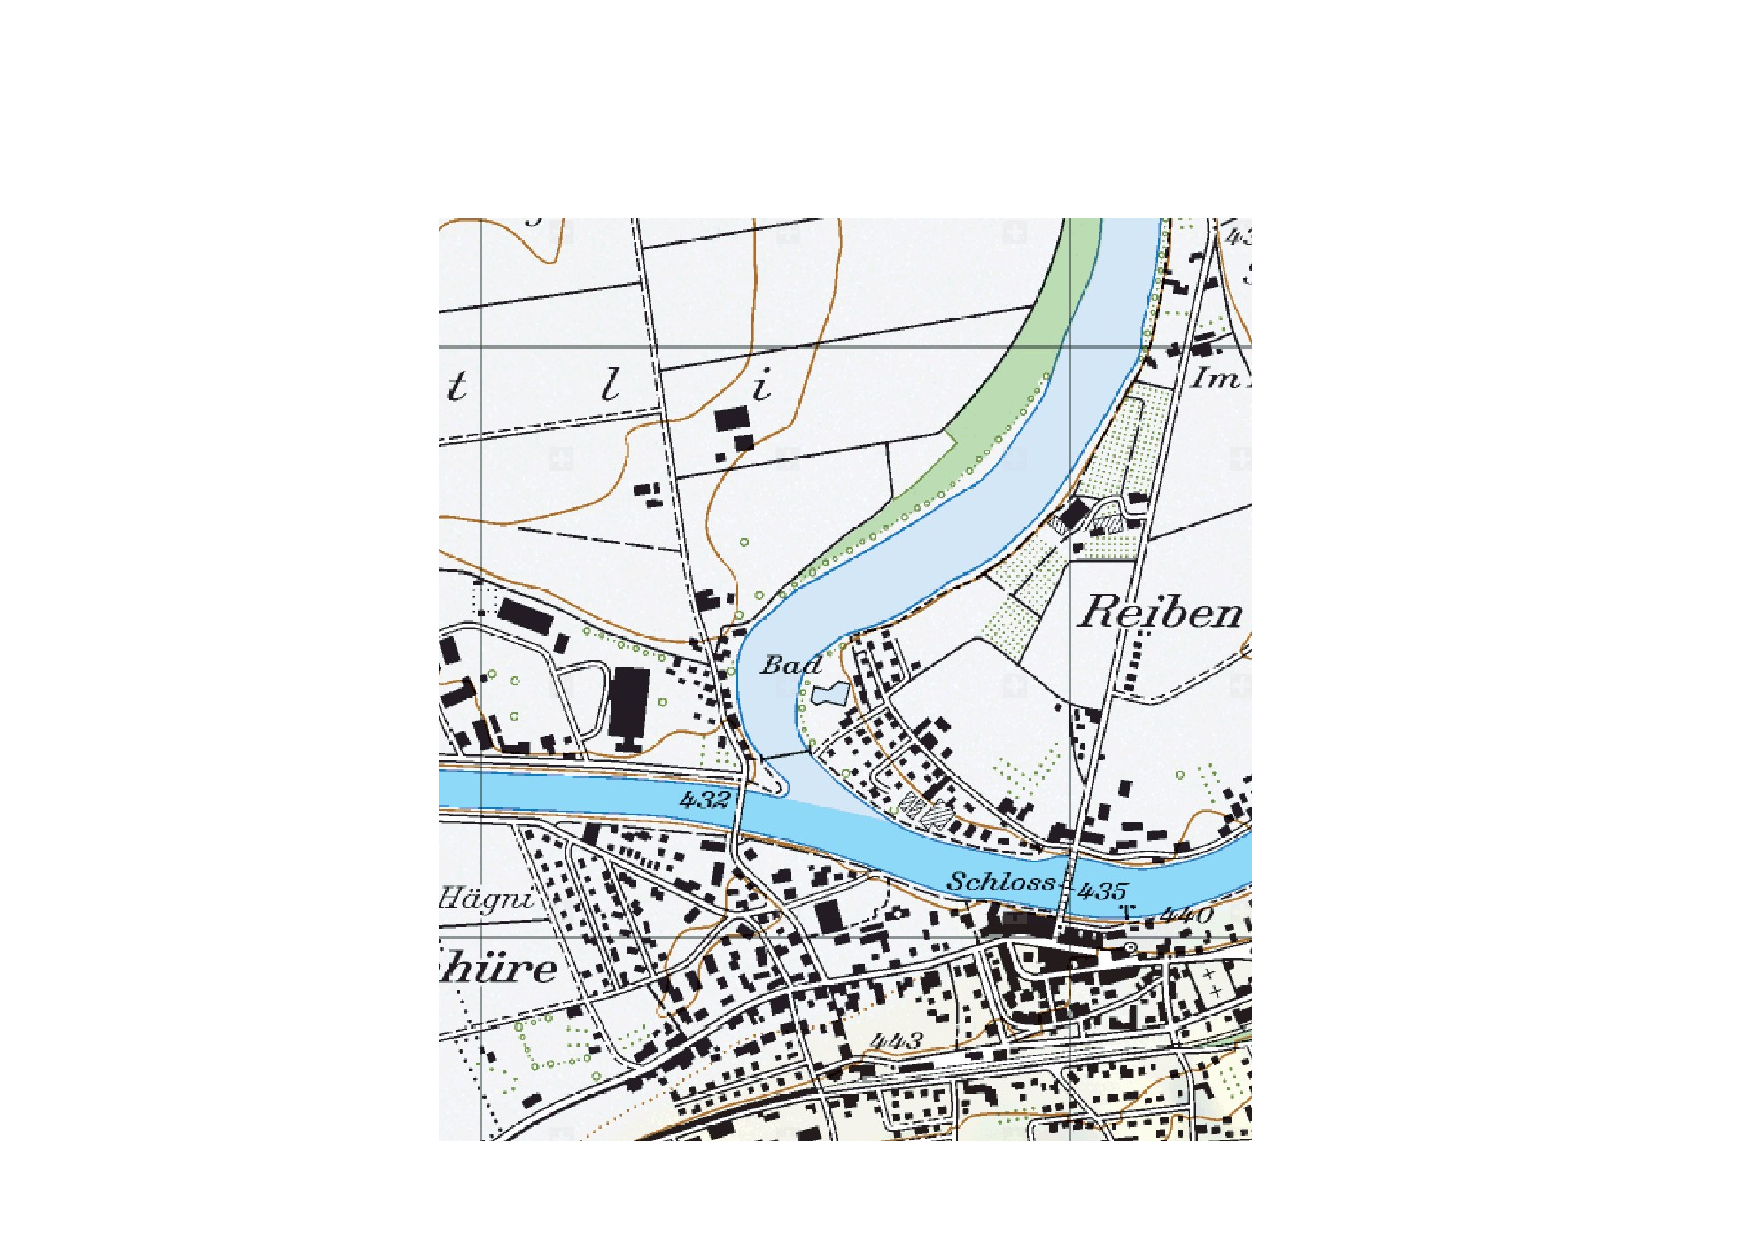
\includegraphics[width=7cm]{pictures/burenmap.pdf}\hspace*{0.2cm}
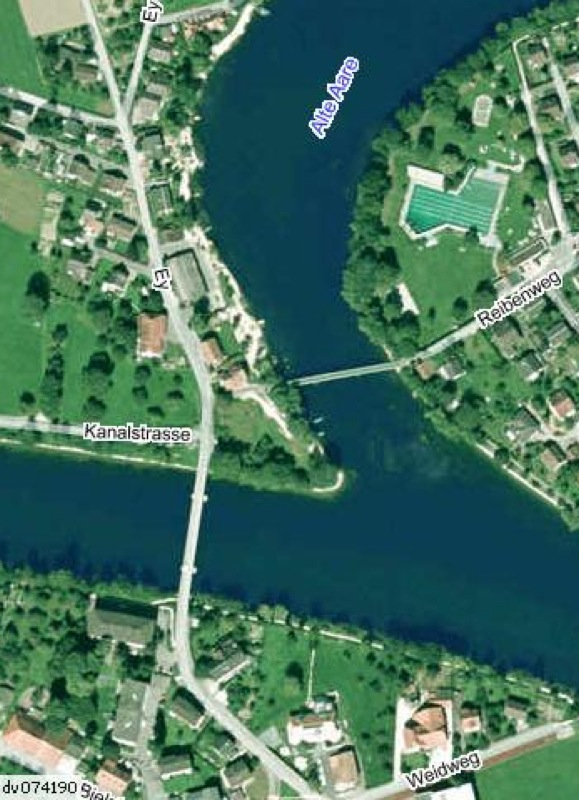
\includegraphics[width=7cm]{pictures/ueb27lb}
\end{center}

\item Der Kreis mit Mittelpunkt $M$ soll von $Z$ aus so gestreckt werden, dass der Bildkreis die Gerade $g$ ber\"uhrt. Konstruiere den Bildkreis.
\begin{center}
\definecolor{qqqqff}{rgb}{0,0,1}
\scalebox{0.9}{
\begin{tikzpicture}[line cap=round,line join=round,>=triangle 45,x=0.7353cm,y=0.7353cm]
\clip(0.52,-6.76) rectangle (16.84,0.36);
\draw [line width=1.6pt] (7.54,-0.4)-- (16.12,-3.18);
\draw [line width=1.6pt] (6.42,-3.68) circle (1.47cm);
\fill [color=black] (6.42,-3.68) circle (1.5pt);
\draw[color=black] (6.16,-3.96) node {$M$};
\fill [color=qqqqff] (0.94,-1.8) circle (1.5pt);
\draw[color=qqqqff] (0.72,-1.4) node {$Z$};
\end{tikzpicture}
}
\end{center}
\item Bei einer zentrischen Streckung eines Kreises vervierfacht sich dessen Radius. Wie ver\"andert sich dabei der Inhalt der Kreisfl\"ache?
\item Bei einer zentrischen Streckung eines Quadrats wird dessen Fl\"acheninhalt $100$ mal gr\"osser. Wie viel mal gr\"osser wird dabei die Seitenl\"ange?
\item Ein Mikroskop vergr\"ossert $100$-fach. Wie viel mal wird mit diesem Mikroskop der Fl\"acheninhalt eines Insektenfl\"ugels vergr\"ossert?
\item Auf einer Karte mit Massstab $1\div25'000$ ist ein horizontales Autobahnst\"uck $\unit[65]{mm}$ lang und eine Stadt bedeckt eine Fl\"ache von $\unit[420]{cm^2}$. Wie lang ist das Autobahnst\"uck und wie gross ist die Stadtfl\"ache in Wirklichkeit?
\item Die Schweiz hat eine Fl\"ache von $\unit[41'000]{km^2}$. Die Luftlinie Bern-Thun betr\"agt $\unit[25]{km}$. Welche Fl\"ache hat die Schweiz auf einer Karte, bei der die Distanz Bern-Thun $\unit[5]{cm}$ betr\"agt?
\item Die Skizze zeigt ein dreieckiges Segel $ABC$, das um eine Stange gewickelt werden kann. Dabei verkleinert sich die Segelfl\"ache auf die gestrichelte Gr\"osse.
\begin{center}
\scalebox{0.8}{
\begin{tikzpicture}[line cap=round,line join=round,>=triangle 45,x=1cm,y=1cm]
\clip(0.52,-4.6) rectangle (6.82,0.36);
\draw [line width=1.6pt] (2.12,-0.24)-- (5.34,-2.86);
\draw [line width=1.6pt] (5.34,-2.86)-- (2.16,-3.34);
\draw [line width=4pt] (2.12,-0.24)-- (2.16,-3.34);
\draw [line width=1.6pt,dash pattern=on 5pt off 5pt] (2.13,-1.12)-- (3.82,-2.48);
\draw [line width=1.6pt,dash pattern=on 5pt off 5pt] (3.82,-2.48)-- (2.15,-2.68);
\draw (1.68,-3.46) node[anchor=north west] {A};
\draw (5.64,-2.76) node[anchor=north west] {B};
\draw (1.5,0.04) node[anchor=north west] {C};
\end{tikzpicture}
}
\end{center}
\begin{enumeratea}
\item Ein Segel von $\unit[20]{m^2}$ Fl\"acheninhalt wird soweit aufgerollt, bis die Segelunterkante $AB$ von $\unit[5]{m}$ auf $\unit[4]{m}$ verk\"urzt wird. Wie gross ist die neue Segelfl\"ache?
\item Ein $\unit[36]{m^2}$ grosses Segel wird auf $\unit[16]{m^2}$ verkleinert. Um welchen Faktor verkleinert sich die Segelunterkante $AB$?
\end{enumeratea}

\pagebreak

\item Die Originalfigur $A$ kann je durch eine \"Ahnlichkeitsabbildung in die Bildfigur $B$, $C$, $D$, $E$, $F$ oder $G$ abgebildet werden.
\begin{center}
\definecolor{zzttqq}{rgb}{0.6,0.2,0}
\definecolor{wwwwww}{rgb}{0.4,0.4,0.4}
\scalebox{0.7}{
\begin{tikzpicture}[line cap=round,line join=round,>=triangle 45,x=1cm,y=1cm]
\draw [color=wwwwww,dash pattern=on 2pt off 2pt, xstep=0.5cm,ystep=0.5cm] (-4.3,-5.24) grid (10.2,6.3);
\clip(-4.3,-5.24) rectangle (10.42,6.3);
\fill[color=zzttqq,fill=zzttqq,fill opacity=0.1] (-3.5,5.5) -- (-0.5,5.5) -- (-0.5,3.5) -- (-1.5,3.5) -- (-1.5,4.5) -- (-3.5,4.5) -- cycle;
\fill[color=zzttqq,fill=zzttqq,fill opacity=0.1] (3.5,3.5) -- (3.5,5.5) -- (6.5,5.5) -- (6.5,4.5) -- (4.5,4.5) -- (4.5,3.5) -- cycle;
\fill[color=zzttqq,fill=zzttqq,fill opacity=0.1] (0.5,2.5) -- (2.5,2.5) -- (2.5,-0.5) -- (1.5,-0.5) -- (1.5,1.5) -- (0.5,1.5) -- cycle;
\fill[color=zzttqq,fill=zzttqq,fill opacity=0.1] (-3,0.5) -- (-1.5,0.5) -- (-1.5,0) -- (-2.5,0) -- (-2.5,-0.5) -- (-3,-0.5) -- cycle;
\fill[color=zzttqq,fill=zzttqq,fill opacity=0.1] (-1.5,-1.5) -- (-0.5,-1.5) -- (-0.5,-3.5) -- (-3.5,-3.5) -- (-3.5,-2.5) -- (-1.5,-2.5) -- cycle;
\fill[color=zzttqq,fill=zzttqq,fill opacity=0.1] (6.5,2.5) -- (9.5,2.5) -- (9.5,1.5) -- (7.5,1.5) -- (7.5,0.5) -- (6.5,0.5) -- cycle;
\fill[color=zzttqq,fill=zzttqq,fill opacity=0.1] (7,-1.5) -- (8.5,-1.5) -- (8.5,-4.5) -- (4,-4.5) -- (4,-3) -- (7,-3) -- cycle;
\draw [color=zzttqq] (-3.5,5.5)-- (-0.5,5.5);
\draw [color=zzttqq] (-0.5,5.5)-- (-0.5,3.5);
\draw [color=zzttqq] (-0.5,3.5)-- (-1.5,3.5);
\draw [color=zzttqq] (-1.5,3.5)-- (-1.5,4.5);
\draw [color=zzttqq] (-1.5,4.5)-- (-3.5,4.5);
\draw [color=zzttqq] (-3.5,4.5)-- (-3.5,5.5);
\draw [color=zzttqq] (3.5,3.5)-- (3.5,5.5);
\draw [color=zzttqq] (3.5,5.5)-- (6.5,5.5);
\draw [color=zzttqq] (6.5,5.5)-- (6.5,4.5);
\draw [color=zzttqq] (6.5,4.5)-- (4.5,4.5);
\draw [color=zzttqq] (4.5,4.5)-- (4.5,3.5);
\draw [color=zzttqq] (4.5,3.5)-- (3.5,3.5);
\draw [color=zzttqq] (0.5,2.5)-- (2.5,2.5);
\draw [color=zzttqq] (2.5,2.5)-- (2.5,-0.5);
\draw [color=zzttqq] (2.5,-0.5)-- (1.5,-0.5);
\draw [color=zzttqq] (1.5,-0.5)-- (1.5,1.5);
\draw [color=zzttqq] (1.5,1.5)-- (0.5,1.5);
\draw [color=zzttqq] (0.5,1.5)-- (0.5,2.5);
\draw [color=zzttqq] (-3,0.5)-- (-1.5,0.5);
\draw [color=zzttqq] (-1.5,0.5)-- (-1.5,0);
\draw [color=zzttqq] (-1.5,0)-- (-2.5,0);
\draw [color=zzttqq] (-2.5,0)-- (-2.5,-0.5);
\draw [color=zzttqq] (-2.5,-0.5)-- (-3,-0.5);
\draw [color=zzttqq] (-3,-0.5)-- (-3,0.5);
\draw [color=zzttqq] (-1.5,-1.5)-- (-0.5,-1.5);
\draw [color=zzttqq] (-0.5,-1.5)-- (-0.5,-3.5);
\draw [color=zzttqq] (-0.5,-3.5)-- (-3.5,-3.5);
\draw [color=zzttqq] (-3.5,-3.5)-- (-3.5,-2.5);
\draw [color=zzttqq] (-3.5,-2.5)-- (-1.5,-2.5);
\draw [color=zzttqq] (-1.5,-2.5)-- (-1.5,-1.5);
\draw [color=zzttqq] (6.5,2.5)-- (9.5,2.5);
\draw [color=zzttqq] (9.5,2.5)-- (9.5,1.5);
\draw [color=zzttqq] (9.5,1.5)-- (7.5,1.5);
\draw [color=zzttqq] (7.5,1.5)-- (7.5,0.5);
\draw [color=zzttqq] (7.5,0.5)-- (6.5,0.5);
\draw [color=zzttqq] (6.5,0.5)-- (6.5,2.5);
\draw [color=zzttqq] (7,-1.5)-- (8.5,-1.5);
\draw [color=zzttqq] (8.5,-1.5)-- (8.5,-4.5);
\draw [color=zzttqq] (8.5,-4.5)-- (4,-4.5);
\draw [color=zzttqq] (4,-4.5)-- (4,-3);
\draw [color=zzttqq] (4,-3)-- (7,-3);
\draw [color=zzttqq] (7,-3)-- (7,-1.5);
\draw (-0.36,5.18) node[anchor=north west] {B};
\draw (3,5.28) node[anchor=north west] {A};
\draw (0.62,3) node[anchor=north west] {C};
\draw (-3.5,0.38) node[anchor=north west] {E};
\draw (6,2.26) node[anchor=north west] {D};
\draw (-0.32,-1.74) node[anchor=north west] {F};
\draw (8.72,-2.08) node[anchor=north west] {G};
\end{tikzpicture}
}
\end{center}
Welche Abbildung ist
\begin{enumeratea}
\item eine Kongruenzabbildung
\item eine Punktspiegelung
\item eine Rotation
\item eine Achsenspiegelung
\item eine Verschiebung
\item eine zentrische Streckung
\end{enumeratea}
\item Welche Figuren sind zueinander \"ahnlich?
\begin{center}
\definecolor{zzttqq}{rgb}{0.6,0.2,0}
\definecolor{zzzzzz}{rgb}{0.6,0.6,0.6}
\scalebox{0.9}{
\begin{tikzpicture}[line cap=round,line join=round,>=triangle 45,x=0.733cm,y=0.733cm]
\draw [color=zzzzzz,dash pattern=on 2pt off 2pt, xstep=0.3665cm,ystep=0.3665cm] (-4.3,1.3) grid (14.8,6.3);
\clip(-4.3,1.3) rectangle (14.8,6.3);
\fill[color=zzttqq,fill=zzttqq,fill opacity=0.1] (-3.5,5.5) -- (-3.5,4) -- (-2.5,4) -- (-2.5,4.5) -- (-3,4.5) -- (-3,5.5) -- cycle;
\fill[color=zzttqq,fill=zzttqq,fill opacity=0.1] (-2,4.5) -- (-1,4.5) -- (-1,2) -- (-1.5,2) -- (-1.5,3.5) -- cycle;
\fill[color=zzttqq,fill=zzttqq,fill opacity=0.1] (0.5,6) -- (0.5,4) -- (4.5,4) -- (4.5,5) -- (2.5,5) -- cycle;
\fill[color=zzttqq,fill=zzttqq,fill opacity=0.1] (0.5,2) -- (0.5,3.5) -- (3.5,3.5) -- (3.5,2.74) -- (2,2.72) -- cycle;
\fill[color=zzttqq,fill=zzttqq,fill opacity=0.1] (5,5.5) -- (7,5.5) -- (7,4.5) -- (6.5,4.5) -- (6.5,5) -- (5,5) -- cycle;
\fill[color=zzttqq,fill=zzttqq,fill opacity=0.1] (6,4) -- (6,2) -- (7,3) -- cycle;
\fill[color=zzttqq,fill=zzttqq,fill opacity=0.1] (7.5,4) -- (9.5,5.5) -- (11.5,4) -- cycle;
\fill[color=zzttqq,fill=zzttqq,fill opacity=0.1] (8,3.5) -- (8.5,3.5) -- (8.5,3) -- (9.5,3) -- (9.5,2.5) -- (8,2.5) -- cycle;
\fill[color=zzttqq,fill=zzttqq,fill opacity=0.1] (11,3.5) -- (11,2.5) -- (14,2.5) -- (14,4.5) -- (13,4.5) -- (13,3.5) -- cycle;
\draw [color=zzttqq] (-3.5,5.5)-- (-3.5,4);
\draw [color=zzttqq] (-3.5,4)-- (-2.5,4);
\draw [color=zzttqq] (-2.5,4)-- (-2.5,4.5);
\draw [color=zzttqq] (-2.5,4.5)-- (-3,4.5);
\draw [color=zzttqq] (-3,4.5)-- (-3,5.5);
\draw [color=zzttqq] (-3,5.5)-- (-3.5,5.5);
\draw [color=zzttqq] (-2,4.5)-- (-1,4.5);
\draw [color=zzttqq] (-1,4.5)-- (-1,2);
\draw [color=zzttqq] (-1,2)-- (-1.5,2);
\draw [color=zzttqq] (-1.5,2)-- (-1.5,3.5);
\draw [color=zzttqq] (-1.5,3.5)-- (-2,4.5);
\draw [color=zzttqq] (0.5,6)-- (0.5,4);
\draw [color=zzttqq] (0.5,4)-- (4.5,4);
\draw [color=zzttqq] (4.5,4)-- (4.5,5);
\draw [color=zzttqq] (4.5,5)-- (2.5,5);
\draw [color=zzttqq] (2.5,5)-- (0.5,6);
\draw [color=zzttqq] (0.5,2)-- (0.5,3.5);
\draw [color=zzttqq] (0.5,3.5)-- (3.5,3.5);
\draw [color=zzttqq] (3.5,3.5)-- (3.5,2.74);
\draw [color=zzttqq] (3.5,2.74)-- (2,2.72);
\draw [color=zzttqq] (2,2.72)-- (0.5,2);
\draw [color=zzttqq] (5,5.5)-- (7,5.5);
\draw [color=zzttqq] (7,5.5)-- (7,4.5);
\draw [color=zzttqq] (7,4.5)-- (6.5,4.5);
\draw [color=zzttqq] (6.5,4.5)-- (6.5,5);
\draw [color=zzttqq] (6.5,5)-- (5,5);
\draw [color=zzttqq] (5,5)-- (5,5.5);
\draw [color=zzttqq] (6,4)-- (6,2);
\draw [color=zzttqq] (6,2)-- (7,3);
\draw [color=zzttqq] (7,3)-- (6,4);
\draw [color=zzttqq] (7.5,4)-- (9.5,5.5);
\draw [color=zzttqq] (9.5,5.5)-- (11.5,4);
\draw [color=zzttqq] (11.5,4)-- (7.5,4);
\draw [color=zzttqq] (8,3.5)-- (8.5,3.5);
\draw [color=zzttqq] (8.5,3.5)-- (8.5,3);
\draw [color=zzttqq] (8.5,3)-- (9.5,3);
\draw [color=zzttqq] (9.5,3)-- (9.5,2.5);
\draw [color=zzttqq] (9.5,2.5)-- (8,2.5);
\draw [color=zzttqq] (8,2.5)-- (8,3.5);
\draw [color=zzttqq] (11,3.5)-- (11,2.5);
\draw [color=zzttqq] (11,2.5)-- (14,2.5);
\draw [color=zzttqq] (14,2.5)-- (14,4.5);
\draw [color=zzttqq] (14,4.5)-- (13,4.5);
\draw [color=zzttqq] (13,4.5)-- (13,3.5);
\draw [color=zzttqq] (13,3.5)-- (11,3.5);
\draw (-4.3,5) node[anchor=north west] {A};
\draw (-1,4) node[anchor=north west] {E};
\draw (1.66,4.8) node[anchor=north west] {B};
\draw (1.12,3.4) node[anchor=north west] {F};
\draw (7,5.34) node[anchor=north west] {C};
\draw (6,3.4) node[anchor=north west] {G};
\draw (9.,4.8) node[anchor=north west] {D};
\draw (8.4,2.6) node[anchor=north west] {I};
\draw (12.7,3.22) node[anchor=north west] {H};
\end{tikzpicture}
}
\end{center}

\pagebreak

\item Wahr oder falsch?
\begin{enumeratea}
\item Alle gleichseitigen Dreiecke sind zueinander \"ahnlich.
\item Alle rechtwinkligen Dreiecke sind zueinander \"ahnlich.
\item Alle gleichschenkligen Dreiecke sind zueinander \"ahnlich.
\item Alle rechtwinklig-gleichschenkligen Dreiecke sind zueinander \"ahnlich.
\item Alle Quadrate sind zueinander \"ahnlich.
\item Alle Rechtecke sind zueinander \"ahnlich.
\item Alle Kreise sind zueinander \"ahnlich.
\end{enumeratea}
\item Sind zwei Vierecke \"ahnlich, wenn die einander entsprechenden Winkel gleich gross sind?
\item Gegeben seien zwei \"ahnliche Dreiecke. Die L\"angen von zwei einander entsprechenden Seiten verhalten sich wie $1\div7$. In welchem Verh\"altnis stehen die Fl\"acheninhalte?
\item Die Fl\"acheninhalte zweier \"ahnlicher Dreiecke verhalten sich wie $4\div25$. Wie verhalten sich die L\"angen von zwei einander entsprechenden Seiten?
\item Die Radien zweier Kreise messen $\unit[7]{cm}$ und $\unit[42]{cm}$. Wie verhalten sich ihre Fl\"acheninhalte?
\item Die Fl\"acheninhalte zweier Quadrate verhalten sich wie $1\div2$. Wie verhalten sich die Seitenl\"angen?

\item Zeigen Sie, dass die gleichschenkligen Dreiecke $ABC$ und $DAB$ in der Gr\"osse von zwei Winkeln \"ubereinstimmen und somit \"ahnlich sind.
\begin{center}
\definecolor{xdxdff}{rgb}{0.49,0.49,1}
\definecolor{zzttqq}{rgb}{0.6,0.2,0}
\definecolor{qqqqff}{rgb}{0,0,1}
\scalebox{0.66}{
\begin{tikzpicture}[line cap=round,line join=round,>=triangle 45,x=1.3cm,y=1.3cm]
\clip(-3.32,-2.02) rectangle (2.84,5.32);
\draw [line width=2pt,color=zzttqq] (-2,-1)-- (1,-1);
\draw [line width=2pt,color=zzttqq] (1,-1)-- (-0.5,4.5);
\draw [line width=2pt,color=zzttqq] (-0.5,4.5)-- (-2,-1);
\draw [line width=2pt] (1,-1)-- (-1.6,0.48);
\fill [color=qqqqff] (-2,-1) circle (1.5pt);
\draw[color=qqqqff] (-2.4,-0.86) node {$A$};
\fill [color=qqqqff] (1,-1) circle (1.5pt);
\draw[color=qqqqff] (1.4,-0.88) node {$B$};
\fill [color=qqqqff] (-0.5,4.5) circle (1.5pt);
\draw[color=qqqqff] (-0.86,4.68) node {$C$};
\fill [color=xdxdff] (-1.6,0.48) circle (1.5pt);
\draw[color=xdxdff] (-1.98,0.6) node {$D$};
\end{tikzpicture}
}
\end{center}

\pagebreak

\item \"Uber der Strecke $AB$ ist der Halbkreis mit dem Mittelpunkt $M$ gezeichnet, $C$ liegt auf dem Halbkreis. Beweise die \"Ahnlichkeit der Dreiecke $ADC$ und $ACB$.
\begin{center}
\definecolor{uququq}{rgb}{0.25,0.25,0.25}
\scalebox{0.8}{
\begin{tikzpicture}[line cap=round,line join=round,>=triangle 45,x=1.4cm,y=1.4cm]
\clip(-0.16,-0.21) rectangle (5.18,5.84);
\draw [shift={(3.61,3.92)},line width=1pt] (0,0) -- (75.63:0.32) arc (75.63:165.63:0.32) -- cycle;
\draw [line width=1pt] (2.68,0.3)-- (3.92,5.14);
\draw [shift={(3.3,2.72)},line width=1pt]  plot[domain=1.32:4.46,variable=\t]({1*2.5*cos(\t r)+0*2.5*sin(\t r)},{0*2.5*cos(\t r)+1*2.5*sin(\t r)});
\draw [line width=1pt] (2.68,0.3)-- (1.5,4.46);
\draw [line width=1pt] (1.5,4.46)-- (3.92,5.14);
\draw [line width=1pt] (1.5,4.46)-- (3.61,3.92);
\fill[line width=1pt] (3.51,4.08) circle (0.02);
\fill [color=black] (2.68,0.3) circle (1.5pt);
\draw[color=black] (3,0.26) node {$A$};
\fill [color=black] (3.92,5.14) circle (1.5pt);
\draw[color=black] (4.3,5.27) node {$B$};
\fill [color=black] (1.5,4.46) circle (1.5pt);
\draw[color=black] (1.1,4.56) node {$C$};
\fill [color=uququq] (3.61,3.92) circle (1.5pt);
\draw[color=uququq] (4,3.99) node {$D$};
\fill [color=uququq] (3.3,2.72) circle (1.5pt);
\draw[color=uququq] (3.7,2.73) node {$M$};
\end{tikzpicture}
}
\end{center}
\item Berechne aus den gegebenen Angaben die Streckenl\"ange $x$.
\begin{enumeratea}
\item \ \\
\begin{center}
\scalebox{0.85}{
\begin{tikzpicture}[line cap=round,line join=round,>=triangle 45,x=1.3739cm,y=1.3739cm]
\clip(-0.16,1.96) rectangle (9.3,5.84);
\draw (0.45,5.1)-- (4.14,2.94);
\draw (4.14,2.94)-- (8.81,5.58);
\draw (0.96,4.8)-- (7.6,4.89);
\draw (2.1,4.13)-- (6.33,4.17);
\draw (1.6,4.7) node[anchor=north west] {$x$};
\draw (3.13,3.8) node[anchor=north west] {3};
\draw (4.8,3.75) node[anchor=north west] {5};
\draw (6.3,4.66) node[anchor=north west] {4};
\draw (4.1,4.4) node[anchor=north west] {$\|$};
\draw (4.23,5.1) node[anchor=north west] {$\|$};
\end{tikzpicture}
}
\end{center}
\item \ \\
\begin{center}
\scalebox{0.8}{
\begin{tikzpicture}[line cap=round,line join=round,>=triangle 45,x=1.2cm,y=1.2cm]
\clip(-0.16,1.96) rectangle (9.3,5.84);
\draw (0.45,2.25)-- (8.54,5.35);
\draw (8.52,3.52)-- (0.01,5.61);
\draw (1,5.68)-- (1,2.11);
\draw (7.8,5.47)-- (7.8,3.24);
\draw (0.32,3.99) node[anchor=north west] {2.8};
\draw (3.42,3.4) node[anchor=north west] {4.5};
\draw (6.54,5.2) node[anchor=north west] {1.8};
\draw (8.07,4.46) node[anchor=north west] {x};
\draw (7.6,4.61) node[anchor=north west] {=};
\draw (0.8,4.45) node[anchor=north west] {=};
\end{tikzpicture}
}
\end{center}
\item \ \\
\begin{center}
\begin{tikzpicture}[line cap=round,line join=round,>=triangle 45,x=1.1cm,y=1.1cm]
\clip(-0.16,-0.47) rectangle (8.29,5.84);
\draw (3.89,4.88)-- (0.34,0.21);
\draw (3.89,4.88)-- (2.92,0.19);
\draw (3.89,4.88)-- (7.48,0.24);
\draw (0.26,0.96)-- (7.27,0.97);
\draw (1.35,2.34)-- (6.33,2.37);
\draw (2.25,2.24) node[anchor=north west] {1.4};
\draw (4.51,2.24) node[anchor=north west] {3.5};
\draw (1.69,0.86) node[anchor=north west] {x};
\draw (4.82,0.84) node[anchor=north west] {4.0};
\draw (3.65,2.6) node[anchor=north west] {$\|$};
\draw (3.34,1.2) node[anchor=north west] {$\|$};
\end{tikzpicture}
\end{center}
\item \ \\
\begin{center}
\begin{tikzpicture}[line cap=round,line join=round,>=triangle 45,x=1.06cm,y=1.06cm]
\clip(0.16,0.94) rectangle (8.65,4.3);
\draw [line width=1pt] (1.17,2.04)-- (7.11,2.01);
\draw [line width=1pt] (7.11,2.01)-- (2.21,3.8);
\draw [line width=1pt] (2.21,3.8)-- (1.17,2.04);
\draw [line width=1pt] (4.89,2.82)-- (4.46,2.03);
\draw (1.75,3.62) node[anchor=north west] {=};
\draw (4.5,2.73) node[anchor=north west] {=};
\draw (1,3) node[anchor=north west] {10};
\draw (2.53,2) node[anchor=north west] {x};
\draw (4.1,2.6) node[anchor=north west] {4};
\draw (5.5,2) node[anchor=north west] {6};
\end{tikzpicture}
\end{center}
\item \ \\
\begin{center}
\begin{tikzpicture}[line cap=round,line join=round,>=triangle 45,x=0.73cm,y=0.73cm]
\clip(0.36,-3.49) rectangle (8.49,3.1);
\draw (1.83,-1.61)-- (6.78,2.76);
\draw (0.66,-0.5)-- (7.25,-2.47);
\draw (4.41,1.18)-- (4.41,-2.16);
\draw (6.18,2.6)-- (6.18,-2.61);
\draw (3.1,-1.4) node[anchor=north west] {x};
\draw (4.46,-0.15) node[anchor=north west] {$5\frac{1}{2}$};
\draw (6.3,0.21) node[anchor=north west] {8};
\draw (5.1,-2) node[anchor=north west] {4};
\draw (4.05,0.42) node[anchor=north west] {=};
\draw (5.85,1.82) node[anchor=north west] {=};
\end{tikzpicture}
\end{center}
\end{enumeratea}
\item Teile, ohne zu messen oder zu rechnen, eine Strecke $AB$ im Verh\"altnis $1\div2$.
\item Konstruiere eine Strecke, f\"ur deren L\"ange $x$ die Beziehung gilt:
\begin{enumeratea}
\item $2\div3=5\div x$
\item $x\div5=3\div4$
\end{enumeratea}
\item Teile, ohne zu messen oder zu rechnen, eine Strecke in vier gleiche Teile.
\item Die Geraden $g$ und $g'$ werden von Parallelen geschnitten. Es sind folgende L\"angen gegeben: $a=\unit[12]{cm}$, $b'=\unit[10]{cm}$, $c=\unit[10]{cm}$, $c'=\unit[12.5]{cm}$. Berechne die fehlenden L\"ange $a'$ und $b$.
\begin{center}
\begin{tikzpicture}[line cap=round,line join=round,>=triangle 45,x=1.2cm,y=1.2cm]
\clip(-4.3,-3.5) rectangle (6.04,6.3);
\draw (-3,3)-- (3.94,5.36);
\draw (-3,-1)-- (5,-2);
\draw (-1,4)-- (-1,-2.24);
\draw (-0.5,4.14)-- (-0.5,-2.28);
\draw (1,4.72)-- (1,-2.18);
\draw (3,5.4)-- (3,-2.18);
\draw (-2.5,3.86)-- (-2.5,-1.48);
\draw (-3.8,3.5) node[anchor=north west] {$g$};
\draw (-3.8,-0.4) node[anchor=north west] {$g'$};
\draw (-2.2,-1.06) node[anchor=north west] {$a'$};
\draw (-2,4.6) node[anchor=north west] {$a$};
\draw (0,5.1) node[anchor=north west] {$b$};
\draw (-0.2,-1.36) node[anchor=north west] {$b'$};
\draw (1.6,5.56) node[anchor=north west] {$c$};
\draw (1.6,-1.52) node[anchor=north west] {$c'$};
\end{tikzpicture}
\end{center}

\pagebreak

\item Die Geraden $g$ und $h$, die sich in $S$ schneiden, begrenzen parallele Strecken. Es sind folgende L\"angen gegeben: $a=\unit[20]{mm}$, $b=\unit[28]{mm}$, $c=\unit[32]{mm}$, $e=\unit[24]{mm}$, $w=\unit[20]{mm}$, $y=\unit[40]{mm}$. Berechne alle fehlenden bezeichneten L\"angen.
\begin{center}
\definecolor{uququq}{rgb}{0.25,0.25,0.25}
\begin{tikzpicture}[line cap=round,line join=round,>=triangle 45,x=0.618cm,y=0.618cm]
\clip(-3.98,-1.58) rectangle (11.41,6.2);
\draw (-3,-1)-- (11,6);
\draw (-2.5,5.5)-- (10.52,-0.5);
\draw (-1.97,5.26)-- (-1,0);
\draw (0,4.35)-- (0.68,0.84);
\draw (6.78,3.89)-- (7.49,0.9);
\draw (7.62,4.31)-- (8.51,0.43);
\draw (10.39,-0.44)-- (9,5);
\draw (-2.87,6.08) node[anchor=north west] {$g$};
\draw (-3.6,-0.53) node[anchor=north west] {$h$};
\draw (-0.92,5.46) node[anchor=north west] {$a$};
\draw (1.91,4.19) node[anchor=north west] {$b$};
\draw (8.25,2.79) node[anchor=north west] {$x$};
\draw (9.83,3.02) node[anchor=north west] {$y$};
\draw (5.2,1.89) node[anchor=north west] {$c$};
\draw (7.3,0.84) node[anchor=north west] {$d$};
\draw (8.8,0.23) node[anchor=north west] {$e$};
\draw[color=black] (-1.21,2.59) node {$u$};
\draw[color=black] (0.56,2.65) node {$v$};
\draw[color=black] (6.7,2.47) node {$w$};
\fill [color=uququq] (4,2.5) circle (1.5pt);
\draw[color=uququq] (3.9,2.92) node {$S$};
\end{tikzpicture}
\end{center}

\item Berechne $u$ und $v$.
\begin{center}
\definecolor{qqqqff}{rgb}{0,0,1}
\definecolor{qqwuqq}{rgb}{0,0.39,0}
\scalebox{0.8}{
\begin{tikzpicture}[line cap=round,line join=round,>=triangle 45,x=0.7cm,y=0.7cm]
\clip(-2.4,-2.95) rectangle (7.7,6.42);
\draw [shift={(6,-2)},color=qqwuqq,fill=qqwuqq,fill opacity=0.1] (0,0) -- (90:0.53) arc (90:180:0.53) -- cycle;
\draw [shift={(2.58,-2)},color=qqwuqq,fill=qqwuqq,fill opacity=0.1] (0,0) -- (90.14:0.53) arc (90.14:180:0.53) -- cycle;
\draw (-2,-2)-- (6,-2);
\draw (6,-2)-- (6,6);
\draw (-2,-2)-- (6,4);
\draw (6,6)-- (0,-2);
\draw (2.57,1.43)-- (2.58,-2);
\fill[color=qqwuqq,fill=qqwuqq,fill opacity=0.1] (5.78,-1.78) circle (0.02);
\draw (-1.46,-2) node[anchor=north west] {$11\;cm$};
\draw (0.88,-2) node[anchor=north west] {$9\;cm$};
\draw (4.16,-2) node[anchor=north west] {$u$};
\draw (2.64,0.12) node[anchor=north west] {$15\;cm$};
\draw (6.08,1.47) node[anchor=north west] {$24\;cm$};
\draw (6.15,5.41) node[anchor=north west] {$v$};
\fill [color=qqqqff] (2.36,-1.8) circle (0.5pt);
\fill [color=qqqqff] (5.8,-1.8) circle (0.5pt);
\end{tikzpicture}
}
\end{center}

\item Gegeben sei ein Quadrat, darin schneiden sich drei Geraden --- wie abgebildet --- in einem Punkt. Berechne $w$, $v$ und $u$.
\begin{center}
\definecolor{zzttqq}{rgb}{0.6,0.2,0}
\scalebox{0.85}{
\begin{tikzpicture}[line cap=round,line join=round,>=triangle 45,x=0.6555232558139537cm,y=0.6555232558139537cm]
\clip(-2.6,4.23) rectangle (8.42,14.03);
\draw [line width=1.2pt,color=zzttqq] (-1,5)-- (7,5);
\draw [line width=1.2pt,color=zzttqq] (7,5)-- (7,13);
\draw [line width=1.2pt,color=zzttqq] (7,13)-- (-1,13);
\draw [line width=1.2pt,color=zzttqq] (-1,13)-- (-1,5);
\draw (-1,11)-- (7,11);
\draw (5,13)-- (-1,5);
\draw (7,5)-- (2.32,13);
\draw (0.49,13.65) node[anchor=north west] {$u$};
\draw (3.58,13.65) node[anchor=north west] {$v$};
\draw (5.5,13.8) node[anchor=north west] {$3\;cm$};
\draw (7,12.45) node[anchor=north west] {$3\;cm$};
\draw (-2.7,12.45) node[anchor=north west] {$3\;cm$};
\draw (7,8.72) node[anchor=north west] {$9\;cm$};
\draw (0.71,11.61) node[anchor=north west] {$w$};
\end{tikzpicture}
}
\end{center}

\pagebreak

\item Berechne die horizontale Entfernung des Kirchturms vom Beobachtungsinstrument.
\begin{center}
\definecolor{xdxdff}{rgb}{0.49,0.49,1}
\definecolor{qqqqff}{rgb}{0,0,1}
\scalebox{0.75}{
\begin{tikzpicture}[line cap=round,line join=round,>=triangle 45,x=1.2cm,y=1.2cm]
\clip(-1.83,2.83) rectangle (10.38,10.57);
\draw [line width=2pt] (-1,4)-- (9,4);
\draw (0,4)-- (-0.01,7.49);
\draw (1,4)-- (0.99,7.47);
\draw (-0.01,7.49)-- (0.25,7.49);
\draw (0.99,7.47)-- (0.75,7.47);
\draw (0.25,7.49)-- (0.52,8.93);
\draw (0.52,8.93)-- (0.75,7.47);
\draw (0.52,8.93)-- (0.52,9.65);
\draw [dash pattern=on 2pt off 2pt] (1,4.72)-- (9.1,4.72);
\draw (8.44,4.72)-- (-0.06,9.76);
\draw [dash pattern=on 2pt off 2pt] (0.52,9.42)-- (8.26,9.43);
\draw [->] (2.99,7.34) -- (3.01,9.42);
\draw [->] (2.99,6.54) -- (3,4);
\draw [dash pattern=on 2pt off 2pt] (0,4.75)-- (-1.01,4.75);
\draw [->] (-0.51,5.35) -- (-0.49,4.75);
\draw [->] (-0.48,3.43) -- (-0.48,4);
\draw [line width=3.6pt] (7,5.58)-- (7,4);
\draw [line width=4.4pt] (8.13,4.9)-- (8.73,4.57);
\draw [->] (8.13,4.9) -- (4.89,6.82);
\draw (-1.17,4.6) node[anchor=north west] {$d=1.5\;m$};
\draw (2.33,7.2) node[anchor=north west] {$h=54\;m$};
\draw (5.6,5.44) node[anchor=north west] {$e=3\;m$};
\draw (7.41,3.9) node[anchor=north west] {$4.5\;m$};
\draw [dash pattern=on 2pt off 2pt] (8.47,4.72)-- (8.47,3.56);
\draw [dash pattern=on 2pt off 2pt] (7,4)-- (6.99,3.54);
\fill [color=qqqqff] (0.52,8.93) circle (1.5pt);
\fill [color=xdxdff] (8.13,4.9) circle (1.5pt);
\end{tikzpicture}
}
\end{center}
\item Visiert man einen vertikal gehaltenen Bleichstift $Z$ zuerst mit dem rechten und dann mit dem linken Auge an, so kommt er mit zwei verschiedenen Gel\"andepunkten $A$ und $B$ zur Deckung. Wie weit ist der Bleistift von $A$ entfernt, wenn der Abstand Bleistift-rechtes Auge $d=\unit[72]{cm}$, Pupillenabstand $s=\unit[7.5]{cm}$ und die L\"ange der Strecke $\overline{AB}=\unit[250]{m}$ bekannt sind?
\item Bern ist $\unit[60]{km}$ von den Alpen entfernt. Wenn man auf der Bundeshaus-Terrasse bei ausgestrecktem Arm abwechselnd mit dem rechten und linken Auge \"uber den Daumen gegen die Alpen blickt, scheint der Daumen vom Eiger zum Jungfraugipfel zu springen. Sch\"atze ihren Augenabstand und den Abstand Auge-Daumen. Wie weit liegen die beiden Berggipfel auseinander?
\item Anna kann mit einem $\unit[7]{cm}$ langen Bleistift, den sie $\unit[35]{cm}$ von ihrem rechten Auge entfernt h\"alt den $\unit[100]{m}$ hohen Berner M\"unsterturm gerade abdecken. Wie weit ist Anna vom M\"unster entfernt?
\item Bei einem gleichschenkligen Trapez messen die parallelen Seiten $\unit[36]{cm}$ und $\unit[60]{cm}$. Die beiden Diagonalen sind je $\unit[60]{cm}$ lang. Berechne die L\"angen der Diagonalabschnitte.
\item Die Basis eines gleichschenkligen Dreiecks misst $\unit[6]{cm}$, die H\"ohe $\unit[12]{cm}$. Dem Dreieck ist ein Quadrat einbeschrieben. Wie lang ist die Quadratseite?
\item Die Sonne erzeugt vom Mond einen Schlagschatten, der als Schattenkegel weit in den Raum hinausreicht. Berechne, wie weit die Spitze des Schattenkegels vom Mondzentrum entfernt ist.
%\begin{center}
%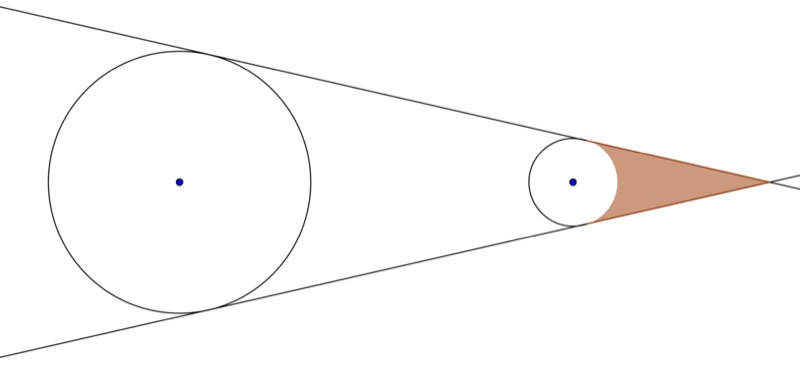
\includegraphics[width=8cm]{ueb59}
%\end{center}

\item Wahr oder falsch?
\begin{enumeratea}
\item W\"urfel sind einander \"ahnlich.
\item Quader sind einander \"ahnlich.
\item Kugeln sind einander \"ahnlich.
\item Zylinder sind einander \"ahnlich.
\end{enumeratea}
\item Ein W\"urfel der Kantenl\"ange $\unit[5]{cm}$ wird mit dem Streckungsfaktor $8$ gestreckt. Welche Kantenl\"ange hat der Bildw\"urfel?

\item Der W\"urfel links wurde von $Z$ aus zentrisch gestreckt.
\begin{center}
\definecolor{qqqqff}{rgb}{0,0,1}
\definecolor{zzzzzz}{rgb}{0.6,0.6,0.6}
\scalebox{0.92}{
\begin{tikzpicture}[line cap=round,line join=round,>=triangle 45,x=0.8cm,y=0.8cm]
\draw [color=zzzzzz,dash pattern=on 2pt off 2pt, xstep=0.475cm,ystep=0.475cm] (-0.73,1.36) grid (15.31,8.78);
\clip(-0.73,1.36) rectangle (15.31,8.78);
\draw (3.5,4)-- (3.5,5);
\draw (3.5,5)-- (4.5,5);
\draw (4.5,5)-- (4.5,4);
\draw (3.5,4)-- (4.5,4);
\draw (3.5,5)-- (3.89,5.36);
\draw (4.5,5)-- (4.88,5.36);
\draw (3.89,5.36)-- (4.88,5.36);
\draw (3.5,4)-- (3.88,4.35);
\draw (4.5,4)-- (4.89,4.35);
\draw (4.88,5.36)-- (4.89,4.35);
\draw (3.89,5.36)-- (3.88,4.35);
\draw (3.88,4.35)-- (4.89,4.35);
\draw (9.5,3)-- (9.5,6);
\draw (9.5,6)-- (12.5,6);
\draw (12.5,6)-- (12.5,3);
\draw (9.5,3)-- (12.5,3);
\draw (9.5,6)-- (10.68,7.08);
\draw (12.5,6)-- (13.63,7.08);
\draw (10.68,7.08)-- (13.63,7.08);
\draw (9.5,3)-- (10.63,4.04);
\draw (9.5,3)-- (10.63,4.04);
\draw (12.5,3)-- (13.68,4.04);
\draw (13.63,7.08)-- (13.68,4.04);
\draw (10.68,7.08)-- (10.63,4.04);
\draw (10.63,4.04)-- (13.68,4.04);
\draw [dotted] (0.5,4.5)-- (3.89,5.36);
\draw [dotted] (3.89,5.36)-- (10.67,7.08);
\fill [color=qqqqff] (0.5,4.5) circle (1.5pt);
\draw[color=qqqqff] (0.35,4.8) node {$Z$};
\end{tikzpicture}
}
\end{center}
\begin{enumeratea}
\item Wie gross ist der Streckungsfaktor?
\item In welchem Verh\"altnis stehen die Kantenl\"angen von Bild- und Originalw\"urfel?
\item In welchem Verh\"altnis stehen die Inhalte der Seitenfl\"achen von Bild- und Originalw\"urfel?
\item In welchem Verh\"altnis stehen die Volumen von Bild- und Originalw\"urfel?
\end{enumeratea}
\item Ein W\"urfel wird zentrisch gestreckt, so dass sich die Kantenl\"angen des Bildw\"urfels zu den Kantenl\"angen des Originalw\"urfels wie $3\div2$ verhalten. Wie verhalten sich
\begin{enumeratea}
\item die L\"angen der K\"orperdiagonalen,
\item die Inhalte der Seitenfl\"achen,
\item die Volumen?
\end{enumeratea}
\item Zwei W\"urfel aus dem gleichen Material wiegen $\unit[1]{kg}$ und $\unit[8]{kg}$. Wie verhalten sich
\begin{enumeratea}
\item ihre Volumen,
\item ihre Kantenl\"angen,
\item die Inhalte ihrer Seitenfl\"achen?
\end{enumeratea}
\item Die Volumen zweier W\"urfel verhalten sich wie $1\div27$. Wie verhalten sich ihre Seitenfl\"acheninhalte?
\item Ein Quader ist $\unit[6]{cm}$ lang, $\unit[4]{cm}$ breit und $\unit[7]{cm}$ hoch. Er wird mit dem Streckungsfaktor $\frac{1}{2}$ zentrisch gestreckt. Welche L\"ange, Breite und H\"ohe hat der Bildquader?
\item

\begin{enumeratea}
\item Die Kantenl\"angen eines Quaders $A$ sind doppelt so lang wie die entsprechenden Kantenl\"angen eines \"ahnlichen Quaders $B$. Wie verhalten sich die entsprechenden Seitenfl\"achen von $A$ und $B$?
\item Die Inhalte der Seitenfl\"achen eines Quaders $C$ sind viermal kleiner als die Inhalte der entsprechenden Seitenfl\"achen eines \"ahnlichen Quaders $D$. Wie verhalten sich entsprechende Kantenl\"angen von $C$  und $D$?
\item Die Kantenl\"angen eines Quaders $E$ sind dreimal kleiner als die entsprechenden Kantenl\"angen eines \"ahnlichen Quadrats $F$. Wie verhalten sich die Volumen von $E$ und $F$?
\item Die Inhalte der Seitenfl\"achen eines Quaders $J$ sind neunmal gr\"osser als die Inhalte der entsprechenden Seitenfl\"achen eines \"ahnlichen Quaders $K$. Wie verhalten sich die entsprechenden Kantenl\"angen von $J$ und $K$?
\item Das Volumen eines Quaders $G$ ist tausendmal gr\"osser als das Volumen eines \"ahnlichen Quaders $H$. Wie verhalten sich die entsprechenden Kantenl\"angen von $G$ und $H$?
\item Das Volumen eines Quaders $L$ ist $64$ mal kleiner als das Volumen eines \"ahnlichen Quaders $M$. Wie verhalten sich die Inhalte entsprechender Seitenfl\"achen von $L$ und $M$?
\end{enumeratea}
\item Die Durchmesser zweier Kugeln verhalten sich wie $4\div5$. Wie verhalten sich ihre Volumen?
\item Die Volumen zweier Kugeln verhalten sich wie $8\div27$. Wie verhalten sich ihre Radien?
\item Zwei Kugeln aus gleichem Material wiegen $\unit[1]{g}$ und $\unit[64]{g}$. Die leichtere Kugel hat einen Durchmesser von $\unit[3]{mm}$. Welchen Durchmesser hat die schwerere Kugel?

\item Eine Kugel wiegt $\unit[16]{kg}$, eine andere aus gleichem Material $\unit[54]{kg}$. Gib in m\"oglichst einfachen ganzen Zahlen an:
\begin{enumeratea}
\item das Verh\"altnis der Volumen,
\item das Verh\"altnis der Durchmesser,
\item das Verh\"altnis der Oberfl\"acheninhalte.
\end{enumeratea}
\item In der Kanalisation einer Siedlung sind die Abflussrohre \"uberlastet. Sie werden durch Rohre mit doppelt so grossem Durchmesser ersetzt. Wie ver\"andert sich das Fassungsverm\"ogen?
\item Die H\"ohe einer quadratischen Pyramide wird durch einen Schnitt parallel zur Grundfl\"ache halbiert. Wie verhalten sich die Volumen
\begin{enumeratea}
\item der Pyramidenspitze und der ganzen Pyramide zueinander,
\item der Pyramidenspitze und des Pyramidenstumpfs zueinander?
\end{enumeratea}
\item In welchem Abstand von der Spitze eines Kegels mit der H\"ohe $h$ muss parallel zur Grundfl\"ache ein Schnitt gelegt werden, wenn das Volumen dadurch im Verh\"altnis $8\div19$ geteilt werden soll?

\item Eine \"agyptische Pyramide mit quadratischem Grundriss wird von waagrecht abgelagertem W\"ustensand allm\"ahlich begraben. Die H\"ohe der noch sichtbaren Pyramide betr\"agt nur noch vier F\"unftel der H\"ohe der urspr\"unglichen Pyramide.
\begin{enumeratea}
\item Wie verhalten sich die Volumen des sichtbaren und des versch\"utteten Teils zueinander?
\item Wie viele $\%$ des urspr\"unglichen Pyramidenvolumens ragen noch aus dem Sand?
\end{enumeratea}

\pagebreak

\item Die beiden massiven K\"orper sind zueinander \"ahnlich und aus gleichem Material.
\begin{center}
\begin{tikzpicture}[line cap=round,line join=round,>=triangle 45,x=1.1319100391134291cm,y=1.1319100391134291cm]
\clip(2.54,1.8) rectangle (14.91,7.28);
\draw [line width=1.6pt] (3.5,5)-- (6,5);
\draw [line width=1.6pt] (3.5,5)-- (3.5,4);
\draw [line width=1.6pt] (3.5,4)-- (6,4);
\draw [line width=1.6pt] (6,4)-- (6,5);
\draw [line width=1.6pt] (6,5)-- (6.5,5.5);
\draw [line width=1.6pt] (6,4)-- (6.5,4.5);
\draw [line width=1.6pt] (6.5,4.5)-- (6.5,5.5);
\draw [line width=1.6pt] (5,6)-- (5.5,6);
\draw [line width=1.6pt] (5.5,6)-- (5.75,6.28);
\draw [line width=1.6pt] (5,6)-- (5.28,6.28);
\draw [line width=1.6pt] (5.28,6.28)-- (5.75,6.28);
\draw [line width=1.6pt] (3.5,5)-- (4,5.5);
\draw [line width=1.6pt] (5,6)-- (3.5,5);
\draw [line width=1.6pt] (5.5,6)-- (6,5);
\draw [line width=1.6pt] (5.75,6.28)-- (6.5,5.5);
\draw [line width=1.6pt] (4,5.5)-- (5.28,6.28);
\draw [line width=1.6pt] (9,3)-- (12.76,3.01);
\draw [line width=1.6pt] (9,3)-- (9,4.5);
\draw [line width=1.6pt] (12.76,3.01)-- (12.76,4.51);
\draw [line width=1.6pt] (12.76,4.51)-- (9,4.5);
\draw [line width=1.6pt] (12.76,3.01)-- (13.49,3.77);
\draw [line width=1.6pt] (12.76,4.51)-- (13.49,5.25);
\draw [line width=1.6pt] (13.49,3.77)-- (13.49,5.25);
\draw [line width=1.6pt] (9,4.5)-- (9.75,5.25);
\draw [line width=1.6pt] (11.5,6)-- (12.25,6.01);
\draw [line width=1.6pt] (12.25,6.01)-- (12.68,6.43);
\draw [line width=1.6pt] (11.5,6)-- (11.99,6.43);
\draw [line width=1.6pt] (11.99,6.43)-- (12.68,6.43);
\draw [line width=1.6pt] (9,4.5)-- (11.5,6);
\draw [line width=1.6pt] (12.76,4.51)-- (12.25,6.01);
\draw [line width=1.6pt] (12.68,6.43)-- (13.49,5.25);
\draw [line width=1.6pt] (9.75,5.25)-- (11.99,6.43);
\draw (5.2,6.8) node[anchor=north west] {4.8};
\draw (2.9,5.51) node[anchor=north west] {8.4};
\draw (4.39,3.89) node[anchor=north west] {13.2};
\draw (6.5,5.2) node[anchor=north west] {7.2};
\draw (8.6,5.2) node[anchor=north] {12.6};
\draw (12.1,6.9) node[anchor=north west] {7.2};
\draw (13.57,4.57) node[anchor=north west] {10.8};
\draw (10.59,2.91) node[anchor=north west] {19.6};
\end{tikzpicture}
\end{center}
\begin{enumeratea}
\item Beim gr\"osseren K\"orper steht eine falsche Zahl. Korrigiere sie.
\item Wie viel wiegt der kleinere K\"orper, wenn der gr\"ossere $\unit[16.2]{kg}$ wiegt?
\end{enumeratea}
\end{enumerate}

\newpage

%\vspace*{-7ex}

\section{Selbstkontrolle}
\begin{enumerate}
\item Zeichne bei der abgebildeten Figur alle Symmetrieachsen ein.
\begin{center}
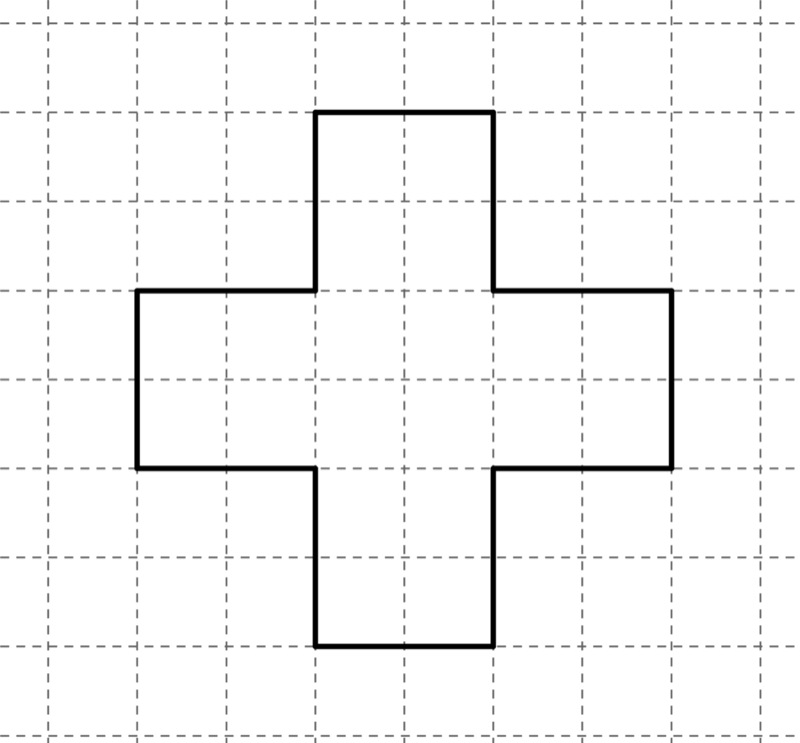
\includegraphics[width=5cm]{pictures/seueb1}
\end{center}
\item Strecke das abgebildete Dreieck vom Punkt $Z$ aus mit dem Streckungsfaktor $2$.
\begin{center}
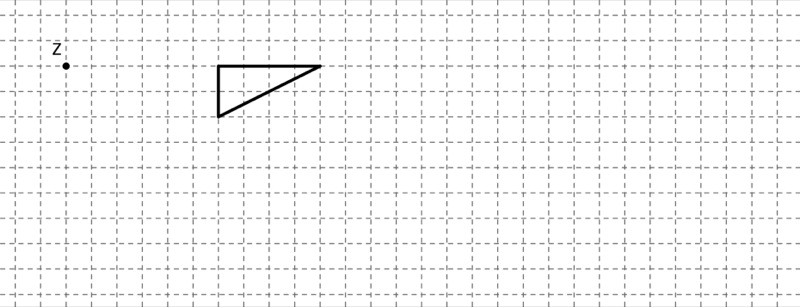
\includegraphics[width=12cm]{pictures/seueb2}
\end{center}
\item Drehe die abgebildete Figur um den Punkt $Z$ um $90^\circ$.
\begin{center}
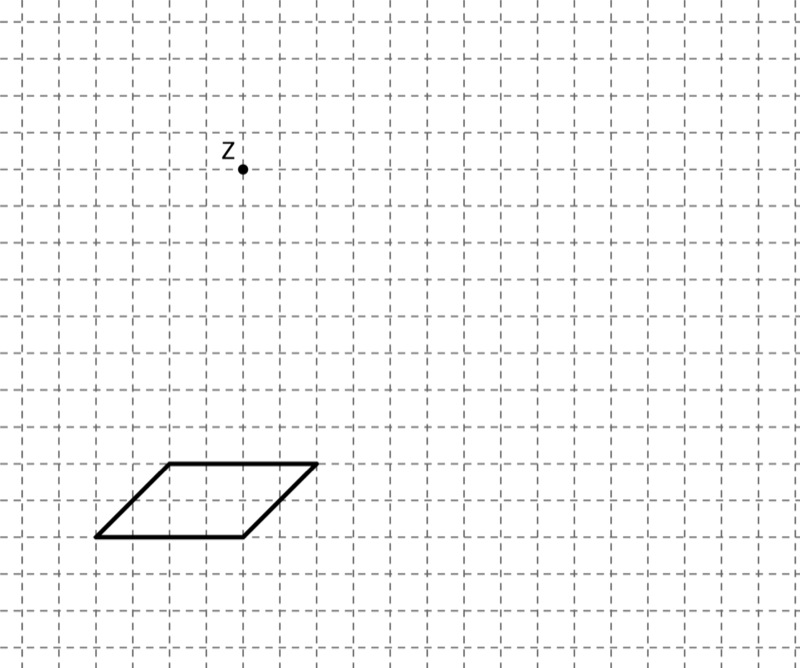
\includegraphics[width=8cm]{pictures/seueb3}
\end{center}

\item Ein gegebenes Dreieck soll von einem gegebenen Punkt aus zentrisch gestreckt werden. Welchen Streckungsfaktor muss man w\"ahlen, um den Umfang des Dreiecks zu vervierfachen?
\item Berechnen Sie die H\"ohe eines Mastes, dessen Schatten eine L\"ange von $\unit[55]{m}$ hat, wenn gleichzeitig der Schatten eines $\unit[180]{cm}$ grossen Mannes $\unit[4.5]{m}$ lang ist.
\item Berechne $x$
\begin{center}
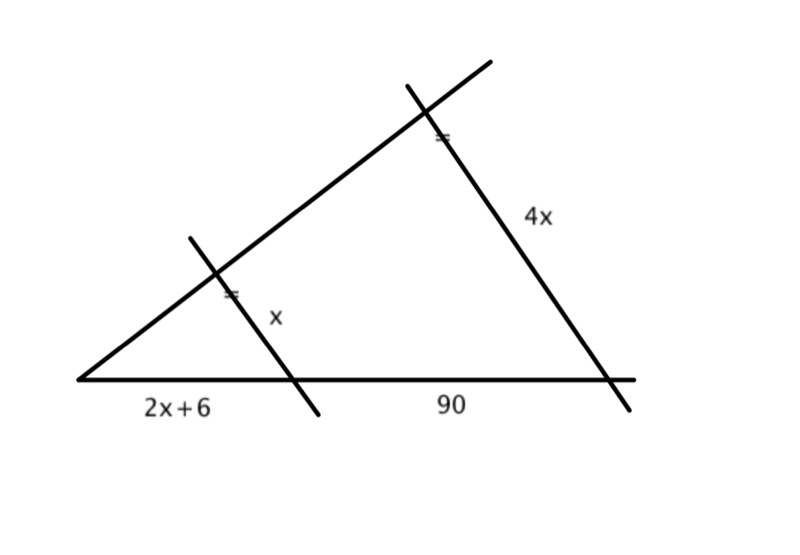
\includegraphics[width=12cm]{pictures/seueb6}
\end{center}
\item Die Durchmesser zweier kugelf\"ormiger Planeten verhalten sich wie $1\div9$. In welchem Verh\"altnis stehen ihre Oberfl\"achen zueinander?
\item Auf einer Karte im Massstab $1\div25\,000$ wird eine Seeoberfl\"ache zu $\unit[416]{cm^2}$ bestimmt. Wie viele Quadratkilometer misst die Seeoberfl\"ache in Wirklichkeit?
\item Ein gerader Kreiskegel wird durch zwei Schnitte parallel zur Grundfl\"ache in drei gleich hohe St\"ucke geteilt. Wie verh\"alt sich das Volumen des obersten zum Volumen des untersten St\"ucks?

\end{enumerate}

\pagebreak

%\section*{L\"osungen}

%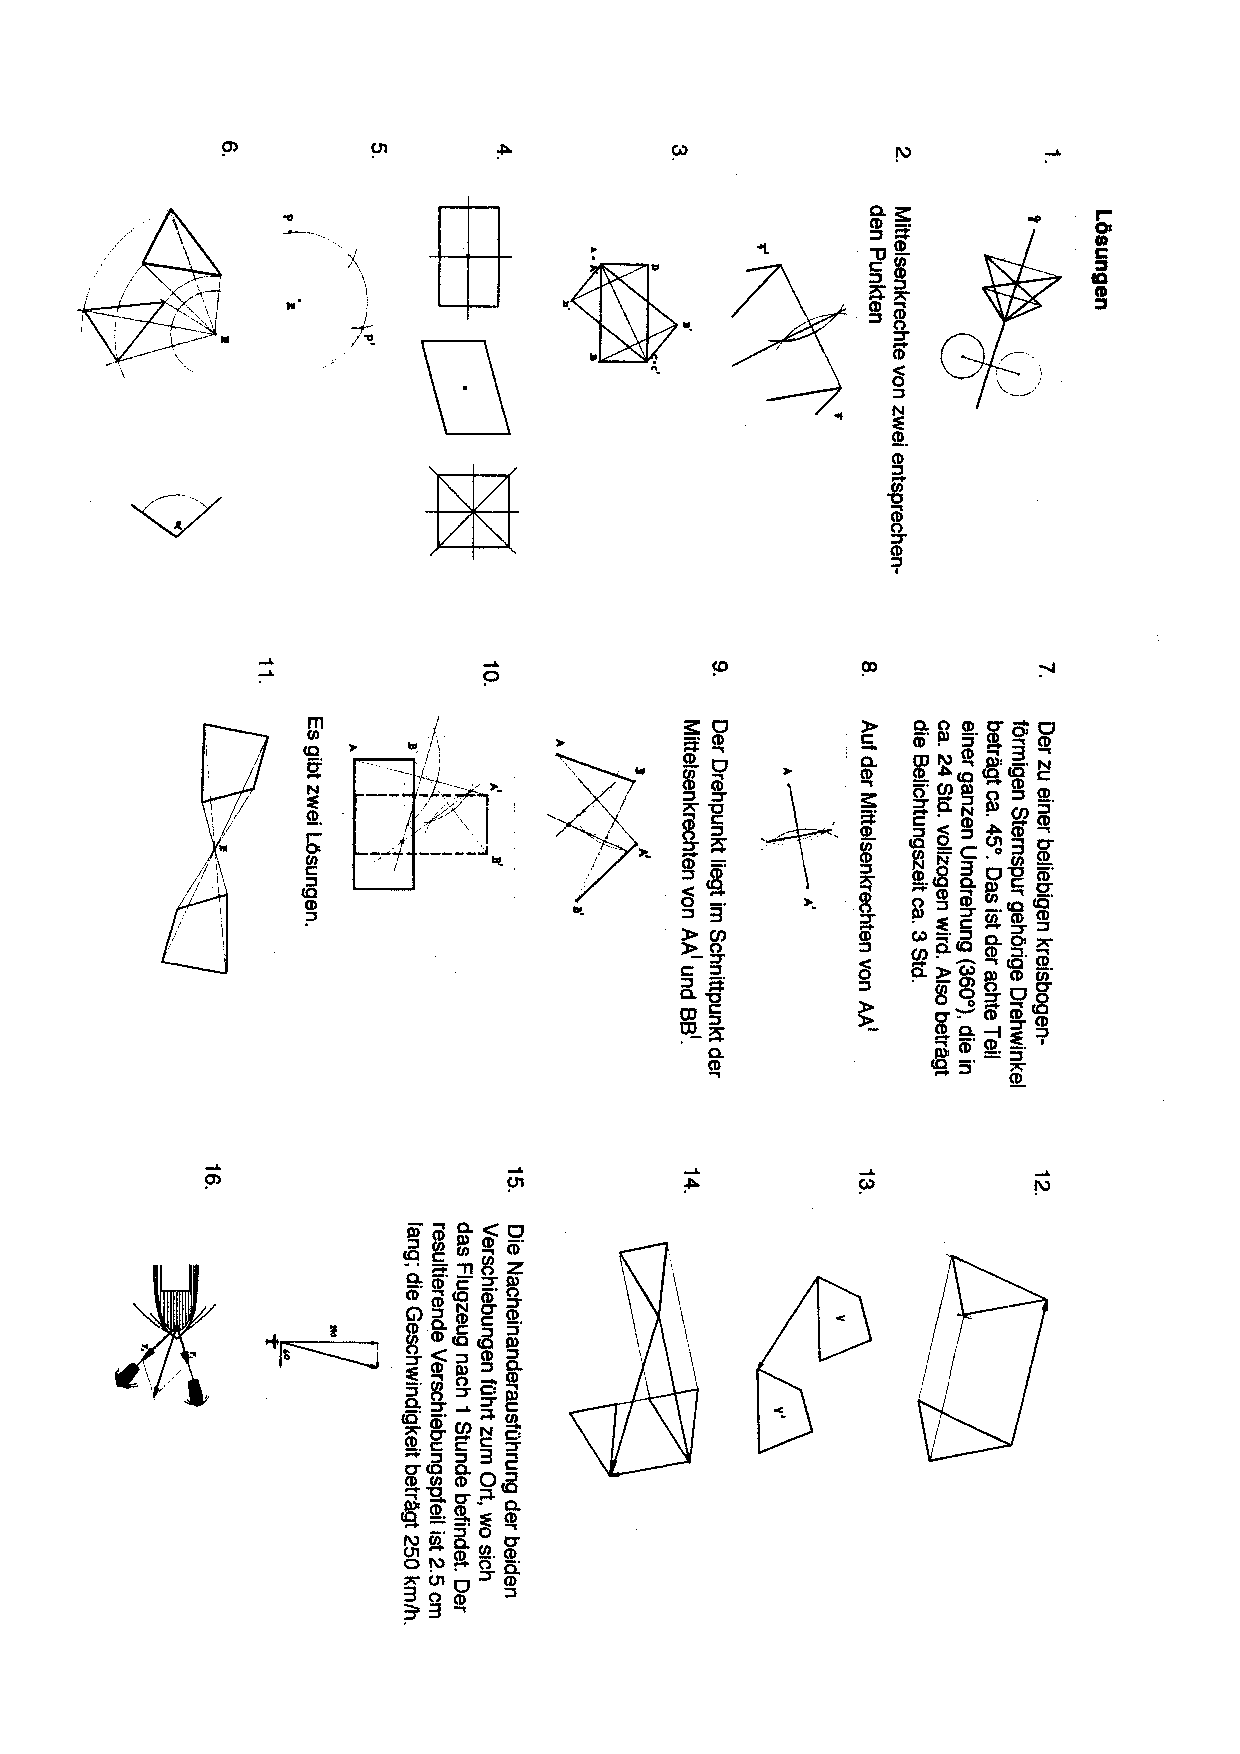
\includepdf[pages={1},scale=.7,pagecommand={}]{aehnlichkeitlsg1}

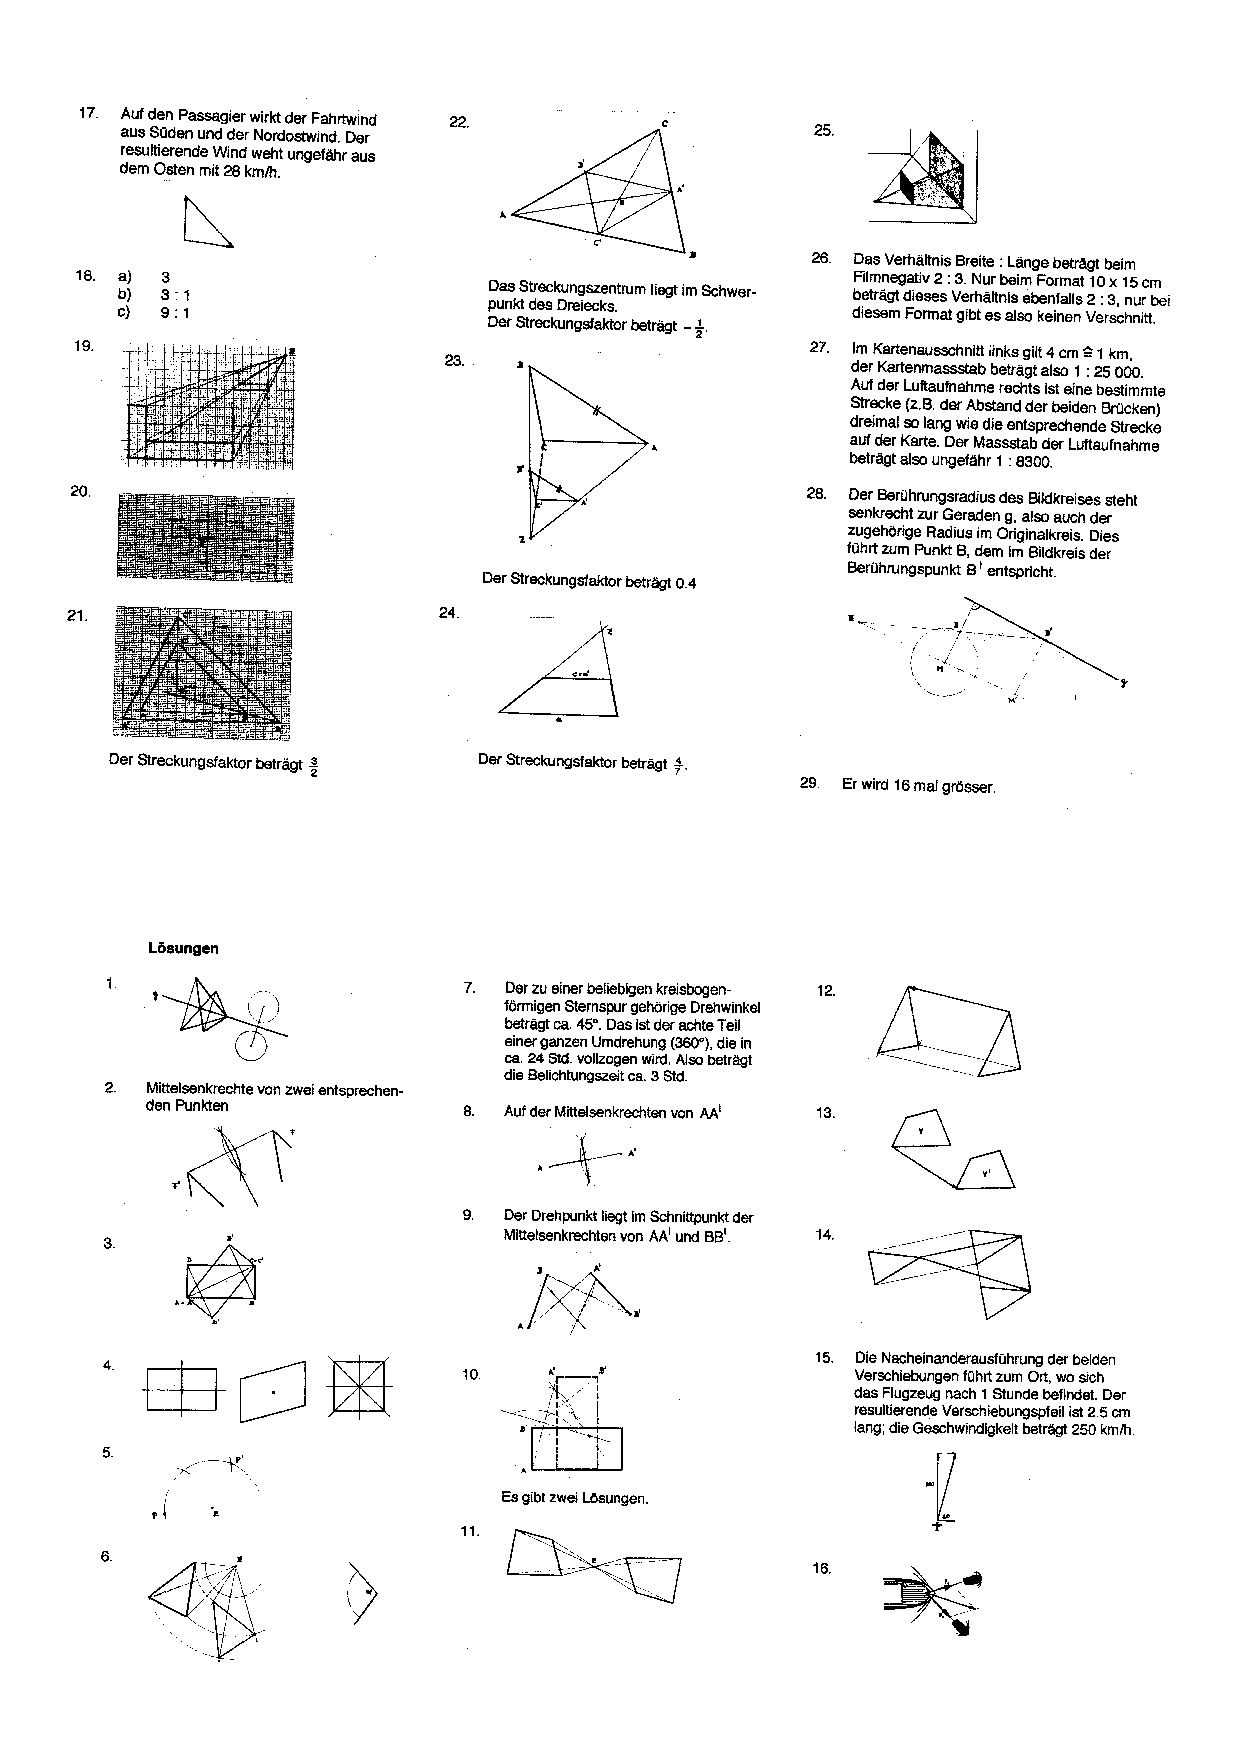
\includepdf[pages={1,2},scale=.7,pagecommand={}]{aehnlichkeitlsg2}

%\clearpage
%\listoffigures
%\listoftables
%\newpage
%\nocite{*}
%\bibliographystyle{plain}
%\bibliography{preamble/literaturgoogle}
\end{document}